% this file is called up by thesis.tex
% content in this file will be fed into the main document

%: ----------------------- introduction file header -----------------------


%------------------------------------------------------------------------- 


% the code below specifies where the figures are stored
%\ifpdf
%    \graphicspath{{Content/figures/PNG/}{Content/figures/JPG/}{Content/figures/PDF/}{Content/figures/}}
%\else
%    \graphicspath{{Content/figures/EPS/}{Content/figures/}}
%\fi
\graphicspath{{ResearchResults/figures/}{ResearchResults/figures/JPG/}{ResearchResults/figures/PDF/}{ResearchResults/figures/}{ResearchResults/figures/EPS/}}

\chapter{Interoperable Architecture for Collaborative Augmented Reality}
\chaptermark{Architecture}
\label{chap:arch}

In this Chapter the \arch{} architecture is presented. \arch{} is an interoperable architecture that simplifies the creation of collaborative AR applications, enables multi-user functionalities and provides advanced mechanisms for data analysis and visualisation. The architecture aims to answer not only the gaps identified in Chapter \ref{chap:sota}, but also to the design objectives identified analysing the answers to a survey completed by 47 primary and secondary school teachers. The architecture has been validated through the development of 3 proofs of concept. \arch{} provides a more mature technological ecosystem that fosters the emergence of AR applications for education and their inclusion in existing school programs.

\section{Overview}\label{sec:introduction}
In recent years, \gls{ar} technology is being used more and more, thanks to an ever-increasing number of devices supporting it, as well as a more mature software ecosystem that allows developers to speed-up the creation of AR-based applications. With their ability to attach virtual content to any physical surface, either through the usage of markers or by using plane detection or geographical information, AR applications have found a valuable role in training and education. Several companies offer educational AR apps and, as detailed in Chapter \ref{chap:sota}, many scientific publications have shown that AR can enhance and improve the learning experience.

Unfortunately though, AR has not yet seen widespread usage in education, and most of the experiences carried out so far are based on small experiments. This is due to several causes (presented in Section \ref{arch:req:surveyres}), which can be summarised with the difficulty for developers and educators to create content that can be used by every student and that integrates well with the existing school curricula. One of the main issues, for example, is that the majority of AR applications available for education provide single-user experiences and they are more apt to be consumed at home rather than at school. Cooperative learning has long been used as an educational approach to improve the learning and performance of the students \citep{Johnson19, kuh2011piecing}, but since the majority of existing AR applications are not multi-user, they do not allow students to cooperate.
Another issue limiting the adoption of AR in schools is the integration of AR applications within existing school programs. Existing applications cannot be easily adapted to specific school curricula, and the data generated inside the apps (e.g., test results or lesson progress) is not automatically added to a \gls{lms}, thus creating additional workload for teachers. 

To solve these problems, a new architecture has been designed. It is called \arch{} (Collaborative Learning Environment for Augmented Reality), and it is an interoperable architecture that enables the creation of multi-user AR applications while providing advanced mechanisms for data analysis and visualisation. This Chapter presents the following contributions:
\begin{itemize}
    \item Definition of multi-user AR requirements and their translation into \glspl{do}. The requirements which an AR-based educational application should satisfy were identified with the help of teachers from an association of Basque primary and secondary schools (Ikastolen Elkartea). They were contacted to complete an online survey. The answers and the feedback provided led to the definition of the requirements and the DOs.
    \item The description of \textit{\ork{}}, a library to support multi-device applications, whose main function is to facilitate the development of this type of apps. \textit{\ork{}} abstracts the communication complexities that arise when trying to develop multi-device applications, and it is the main component of \arch{}.
    \item An interoperable architecture for multi-user AR-based apps. \arch{} is an architecture that allows educators and developers to design multi-user and collaborative learning experiences. Multi-users interaction allows sharing the same AR experience across users as well as transmission of information of any kind (textual, audio, video or 3D). This information could be, for example, interactions of a student in the augmented space, data gathered by the sensors in the devices, information provided by the professor from his laptop or a live video grabbed by a user with their mobile phone. \arch{} also includes libraries for data analysis and data modeling. As it has been designed with ease of use as one of the core \glspl{do}, the architecture offers the user several web-based tools for data visualisation, reporting and information sharing. As the availability of hardware and software is extremely heterogeneous across different schools, the architecture supports several platforms, both web and native.
    \item Validation of the \glspl{do} within the proposed architecture. Three \gls{poc} applications were developed to perform an initial validation of the architecture (which is further validated with end-users as described in Chapter \ref{chap:eval}). Such PoCs are released as open-source software\footnote{\url{https://github.com/Stocastico/ARchitecture_paper}} and can be used and combined by developers to create their own AR applications. These \glspl{poc} do not include all functionalities required by full-fledged applications: for example, privacy considerations such as compliance to GDPR (or other national or local regulations), user handling or access right management are not included in the PoCs, as such functionalities are application dependent and can vary greatly depending on the scope of the app.
\end{itemize}

The rest of this Chapter is organised as follows: Section \ref{arch:related} presents the related work. Section \ref{arch:requirements} describes the requirements of a multi-user AR architecture, how they were collected and how they are translated into design objectives, while Section \ref{arch:architecture} introduces \arch{}. Section \ref{arch:implementation} presents the PoCs implemented to validate \arch{} and, finally, Section \ref{arch:conclusions} summarises the Chapter.

%%%%%%%%%%%%%%%%%%%%%%%%%%%%%%%%%%%%%%%%%%%%%% RELATED

\section{Related work}\label{arch:related}

In the last few years, a massive amount of publications presented implementations of AR applications for education (see Chapter \ref{chap:sota}). The review of Phon et al. (\citeyear{6821833}) is of special interest as it describes ten collaborative AR applications used in education. Of the ten studies, only four include collaborative features in the AR experience, while the others only use the collaborative approach as a learning strategy, which is not reflected in the application.

As the support of AR technology in modern browsers is relatively recent, there is a scarcity of publications presenting web-based AR applications. 
The work of Abriata (\citeyear{abriata2020building}) describes a web application based on a client-server architecture. It enables the creation of AR experiences for molecular visualisation, while \cite{coma2019fi} present a solution for the creation and visualisation of generic AR applications in browsers which uses the FIWARE open-source software framework.

Even though most educational AR applications described in the literature are intended to be single-user, researchers have been investigating collaborative AR experiences since the seminal publication of Billinghurst et al. (\citeyear{billinghurst2002collaborative}). In \cite{lopez2020emofindar}, the authors present a markerless AR application for improving socialization and communication skills of primary school children, and note that the collaborative game version of the app has a greater impact on emotional affection and social interaction. Oh et al. (\citeyear{oh2017hybrid}) describe a collaborative AR app where the user, through the use of smart glasses, can study properties of light such as reflection and refraction.

Besides AR, the revolution of Information and Communication Technologies (ICT) has affected education in many other ways, providing means to enhance both the teaching and learning processes. Nowadays,  \gls{tel}, such as \glspl{its}, Adaptive
Hypermedia Systems (AHSs), and Learning Management Systems (LMSs), are being widely used in many  schools and becoming essential for education. 
An \gls{its} is a system which aims to replicate with digital tools the effectiveness of human tutoring. Even though the first ITS was created over 50 years ago \citep{carbonell1970ai}, recent advances in \gls{ai} translated into the development of newer systems for both education and professional settings \citep{mousavinasab2021intelligent} that have an effectiveness comparable to that of human tutoring \citep{doi:10.1080/00461520.2011.611369}. The architecture of an ITS is typically composed of four components: a Domain model, a Student model, a Tutoring model and a User Interface \citep{nkambou2010advances}. AI tools can be applied to each model but are especially relevant for Student models, as they represent the current state of knowledge of the students and are used to provide optimal teaching interventions \citep{SEDLMEIER20017674}. Student models can then be characterized by what kind of information they model and how this information is stored and used \citep{CHRYSAFIADI20134715}. There are only a few studies examining the combination of \glspl{its} architectures and AR: in \cite{westerfield2015intelligent} the authors present an AR application for motherboard assembly, where the usage of an ITS allows personalized training, while the work of Sanchez-Sobrino et al. (\citeyear{app10041518}) uses AR to create 3D graphical representations of computer programs, helping students learn new programming concepts.

\gls{vla} is the research area at the intersection of Visual Analytics and Learning Analytics \citep{Theron2020}. A recent survey of studies applying VLA to educational settings shows that so far there are very few examples of bringing VLA tools into the classroom and they generally use only very simple visualisations and do not consider background student information as data source \citep{VIEIRA2018119}. Another review study \citep{bodily2018open} analyses similarities and differences between \glspl{olm} and \glspl{lad} and concludes that there is a strong overlap in the two fields, and that applying the lessons learned in OLM research can drive the next generation of learning analytics tools. 

Despite the huge amount of literature describing AR applications for education, there are currently no works describing systems and architectures that use AR technology, provide multi-user and collaborative functionalities and make use of \gls{vla} tools and/or \glspl{its}.

%%%%%%%%%%%%%%%%%%%%%%%%%%%%%%%%%%%%%%%%%%%%%% REQ

\section{Requirements and design objectives}\label{arch:requirements}

To better understand the requirements of an architecture that enables educators to easily incorporate collaborative AR applications in their curricula, a questionnaire for teachers of primary and secondary education level was prepared. In the questionnaire, the teachers were asked a set of questions related to the usage of technology, and AR in particular, in their schools. The survey followed the methodology recommended in \citep[Chapter~5]{lazar2017research}, and it was later modified following the recommendations of the teachers who revised the document. They suggested to reduce the amount of open-ended questions and to prepare a survey which would not take more than 20 minutes to fill. Based on the answers to the survey, a set of requirements was extracted, which in turn defined the \glspl{do} of the proposed architecture. 

\subsection{Teacher survey}\label{sec:req:survey}

The teacher survey, presented in Appendix \ref{append:teachsur}, is composed of 45 questions, split across 3 sections. 19 of the questions are open-ended and in many cases optional, while the remaining questions are multiple choice.
The respondents did not have to answer all the questions, since the survey presented different branching paths based on the answers provided. For example, there is a set of questions asking about the teachers experience with AR applications, which are presented only to the respondents who answered positively in the question about the previous usage of AR in the classroom.   

The first section of the survey contains 16 questions about the teachers (which subjects they are teaching, their years of experience, whether they teach in primary or secondary schools, etc.) and about the generic usage of technology in the classroom (how many laptops, tablets or smartphones are available at school, what applications they use besides office-related or videoconferencing solutions) and what advantages are provided by such technologies.

The second section contains 14 questions specific to the usage of AR applications at school. The section starts with a brief description of what AR is, as well as a few examples of how AR applications can be used in schools. These paragraphs were introduced so that even lecturers not familiar with the technology would be able to answer the questions related to AR. If the teachers had already used AR, the survey asked how often they used it, what they needed to use it, on which devices and whether they were satisfied with the experience. If the teachers did not have any previous experience using AR at school, the survey asked them whether they thought that AR could be a valuable tool to facilitate learning.
Furthermore, the questionnaire asked the teachers what changes would be required in order to improve the experience of using AR and whether they think that an AR-based application would improve the  learning experience of the students.

The final section includes 15 questions about the technological tools the teachers would like to use in their daily activities and when and where they would like to use them. Some questions focused specifically on AR, its advantages and disadvantages, what the teachers consider as the most interesting functionalities of AR apps, what kind of content they would show in the app and their willingness to create such applications, if they were given adequate authoring tools. The final questions were about the usage of AR in a collaborative learning environment and about the inclusion of AI as a support tool for analysing student data and creating automatic reports.

\subsection{Survey results}\label{arch:req:surveyres}

The survey was answered by 47 teachers belonging to Ikastolen Elkartea, a Basque association of primary and secondary schools. In this subsection, the results of the survey are briefly summarised. The answers from the teachers were used to define the architecture requirements. The collection of anonymised answers, together with an exploratory data analysis, is available online\footnote{\url{https://anon.to/3vzfK4}}.

With respect to demographic information, the majority of the respondents (53\%) teaches STEM subjects in secondary schools (82\%), in classes with 25 students on average. 43\% of the teachers who answered the survey are \textit{facilitators}, i.e., teachers in charge of helping colleagues to use technical tools in the classroom, and they are usually the most tech-savvy  among the school personnel.

Schools are usually provided with many computers: although there is a lot of variance across the answers provided, on average each school has 68 desktop PCs available as well as 398 laptops. Tablets are seldom used (42\% of the teachers said they have no tablets in school, but others mentioned an availability of up to 75 tablets). Every teacher mentions they have mobile devices available, but in most cases only their personal device. Teachers also mentioned that most of the students have a personal device, depending on their age (which was not asked in the survey). Apart from this, the teachers mentioned that they often use devices such as Chromebooks or Ultrabooks, digital blackboards, projectors or Apple TVs. From this, a solution that will work on top of different platforms and devices is extracted as a requirement (Requirement 1 - \textbf{R1}).

Regarding software, 77\% of the respondents use software tools (besides Office applications) every school day. The most used applications are Moodle, the Google suite (Classroom, Drive, YouTube, Earth, Maps), SketchUp, Scratch, GeoGebra, Prezi and Lucidpress. The teachers use these applications because they help motivate the students and achieve teaching objectives. The most appreciated aspects of these applications are (in descending order):
\begin{itemize}
        \item They provide services which are accessible from different devices (86\% of the respondents) (\textbf{R1}).
        \item Foster the interaction between the teacher and the students (86\%) (\textbf{R2}).
        \item Foster the interaction between multiple students (75\%) (\textbf{R3}).
        \item Provide customisation options (language, content, etc.) (69\%) (\textbf{R4}).
        \item Gather data on how the application was used (53\%) (\textbf{R5}).
\end{itemize}

Apart from these aspects, the teachers underlined as relevant aspects the possibility to update and maintain the tools (both hardware and software), providing the tools for free and using hardware with enough storage capacity (\textbf{R6}).

Regarding AR, the vast majority of the respondents (88\%) never used it at school, and only about 3\% used it more than once and very seldom. The question specifically mentions the usage of AR in school, and the high percentage does not reflect the familiarity of the teachers with the technology or their usage of AR in other contexts. Among those who used it, 75\% of the teachers think that AR improved the learning process of the students. Despite the low usage of AR technology, 78\% of the teachers think that AR can be a very useful tool. When asked what could help in increasing AR adoption in schools, about 75\% of the teachers emphasized they would need to know the existing AR ecosystem better, what apps are available and their capabilities. Half of the teachers said that they would need more time and to have better hardware and software available for the students (\textbf{R7}). Other answers mentioned the necessity of technical support, better localization of the content and the ability to support multi-user interactions (\textbf{R8}), as the students get bored fairly soon doing individual activities. In general, teachers are dissatisfied with AR for education, rating it 2.2 on a Likert scale (where 1 means \textit{very low satisfaction} and 5 means \textit{very high}). The reasons for this is because most of the AR apps are very limited in terms of interactivity and user experience, and there is nearly no content in the Basque language. Despite this, 70\% of the respondents think that AR can be of added value in learning, and the remaining 30\% think that it may be. The main advantages of AR, as identified by the teachers, are:
\begin{itemize}
        \item Improvement of the motivation of the students (82\%).
        \item Better assimilation of concepts (78\%).
        \item Better way to transfer knowledge (69\%).
        \item Improvement of spatial orientation (58\%).
        \item Improvement of interactivity (49\%).
\end{itemize}

On the other hand, the teachers identified several key limitations of AR, as it requires an effort to learn how to use the technology and the school curricula must be adapted to include it. Furthermore, teachers often lack the time to get familiar with the technology and the experience is often not engaging enough, either because the devices used are too old or because the apps lack content. Ideally, the teachers would like to use AR applications that:
\begin{itemize}
        \item Enable collaboration between multiple students as well as with the teacher.
        \item Are highly interactive and with plenty of quality content.
        \item Can work with a broad range of devices.
        \item Can be used both in the classroom and remotely.
        \item Collect data about how the students used the app.
\end{itemize}

The teachers also expressed interest in having the possibility to create their own AR content, if they were provided an authoring tool and training on how to use it. More than half of the respondents (53\%) expressed their interest and that they would like to create simulations, quiz activities, immersive videos and 3D visualisations. Some of them mentioned that they routinely use tools such as Kahoot\footnote{\url{https://kahoot.com/}} for creating interactive web quizzes and they could use something similar for the creation of AR experiences.

Finally, regarding the usage of \gls{ai} in education, 40 teachers identified the following use cases:
\begin{itemize}
        \item Analysis of usage data and usage patterns (63\%) (\textbf{R9}).
        \item Automatic analysis of the difficulty of the questions in a test-type activity (60\%) (\textbf{R10}).
        \item Identification of students with difficulties at an early stage (58\%) (\textbf{R11}).
\end{itemize}

Table \ref{arch:tab:summaryreqs} recapitulates all the architecture requirements identified after analysing the answers to the survey.

\begin{table*}[ht]\centering
%\renewcommand{\arraystretch}{1.1}
\caption{\fontsize{10pt}{11pt}\selectfont{\itshape{Summary of the requirements identified from the results of the teacher survey.}}}
\begin{tabular}{p{0.1\textwidth}>{\arraybackslash}p{0.78\textwidth}}
\toprule
Code & Requirement\\
\midrule
R1 & Apps should work on different platforms and devices\\
R2 & Foster teacher-student interactivity\\
R3 &  Foster student-student interactivity\\
R4 & Enable several customisation options\\
R5 & Collect data on how the applications are used\\
R6 & Enable easy development as well as installing and updating\\
R7 & Apps should work smoothly even on older hardware\\
R8 & Apps should allow collaborative work\\
R9 & Provide tools for analysis of data and usage patterns\\
R10 & Enable automatic analysis test difficulty \\
R11 & Detect students with learning difficulties \\
\bottomrule
\end{tabular}
\label{arch:tab:summaryreqs}
\end{table*}

\subsection{Design objectives}\label{arch:req:desobj}

Based on the answers of the teachers collected in the survey and the identified requirements, six \glspl{do} (summarised in Figure \ref{fig:desobjs})  were derived. They guide the definition of an architecture for AR-based applications which can be used in schools.

The architecture must be \textbf{interoperable} (\textbf{DO1}). It should run on different devices such as \glspl{hmd}, tablets, laptops or smartphones, with reasonable support for older models. At the software level, the architecture should provide \glspl{api} for development on native platforms (Android and iOS), for cross-platform engines like Unity and support Web standards for \gls{xr} experiences \citep{Goregaokar:22:WDA} and real time communication \citep{rfc7478}. An interoperable architecture has two advantages: it eases the dependence on specific hardware, thus reaching a wider user base, and it allows the development of hybrid solutions where users can connect either using an app or their browser.

The architecture should support \textbf{multi-user interactions} (\textbf{DO2}), both face-to-face and remote. Collaboration is a key requirement identified by teachers to increase the engagement of the students and keep them interested, so the architecture should enable user communication (via voice or chat) and also provide a way to exchange any kind of data in real-time, for example the interactions of the users with the application, the position of the AR camera, the answers to the questions in the app, etc.

The architecture should enable \textbf{long-term storage} (\textbf{DO3}) of the data collected, to guarantee that the teachers can track the progress of the students over time and to let them create \textbf{data visualisations} or automatic reports (\textbf{DO4}). The data will enable the implementation of \textbf{AI techniques} (\textbf{DO5}). The architecture gathers information about how the students are using the applications (both the interactions with the software as well as with other users) and store it in the appropriate format. The architecture should be agnostic to the AI models built on top of it (depending on the application, teachers may be interested in using recommender systems, anomaly detection systems or clustering algorithms, for example) but it should provide support for training a model from scratch, fine-tuning a previously trained model or using an existing model for inference tasks.

Finally, it should be \textbf{easy to develop} content using the specified architecture (\textbf{DO6}). Simplifying the development process would hopefully encourage developers to create applications based on the architecture, thus solving the problem of the lack of quality content identified by the teachers. The architecture should also be \textbf{easy to use}, simplifying the deployment and maintaining of the apps: in the ideal case the teacher using the AR application would be able to install and update the software for himself and the students without the need of external help. It should be noted though, that this design objective is not geared toward the creation of an authoring tool but rather on the definition of a set of libraries and APIs that allow software developers to speed up the app creation process. There is a lack of teacher-oriented authoring tools: most of them have been developed for computing literate users or software engineers and, therefore, they become too complicated for teachers, who may give up the development of their own applications. Brusilovsky et al. (\citeyear{brusilovsky2003adaptive}) claim that teachers should focus on Domain Module authoring while the development of the core of technology support learning systems should be carried out by expert developers.

\begin{figure*}[htbp]
    \centering
    %\captionsetup{justification=centering}
    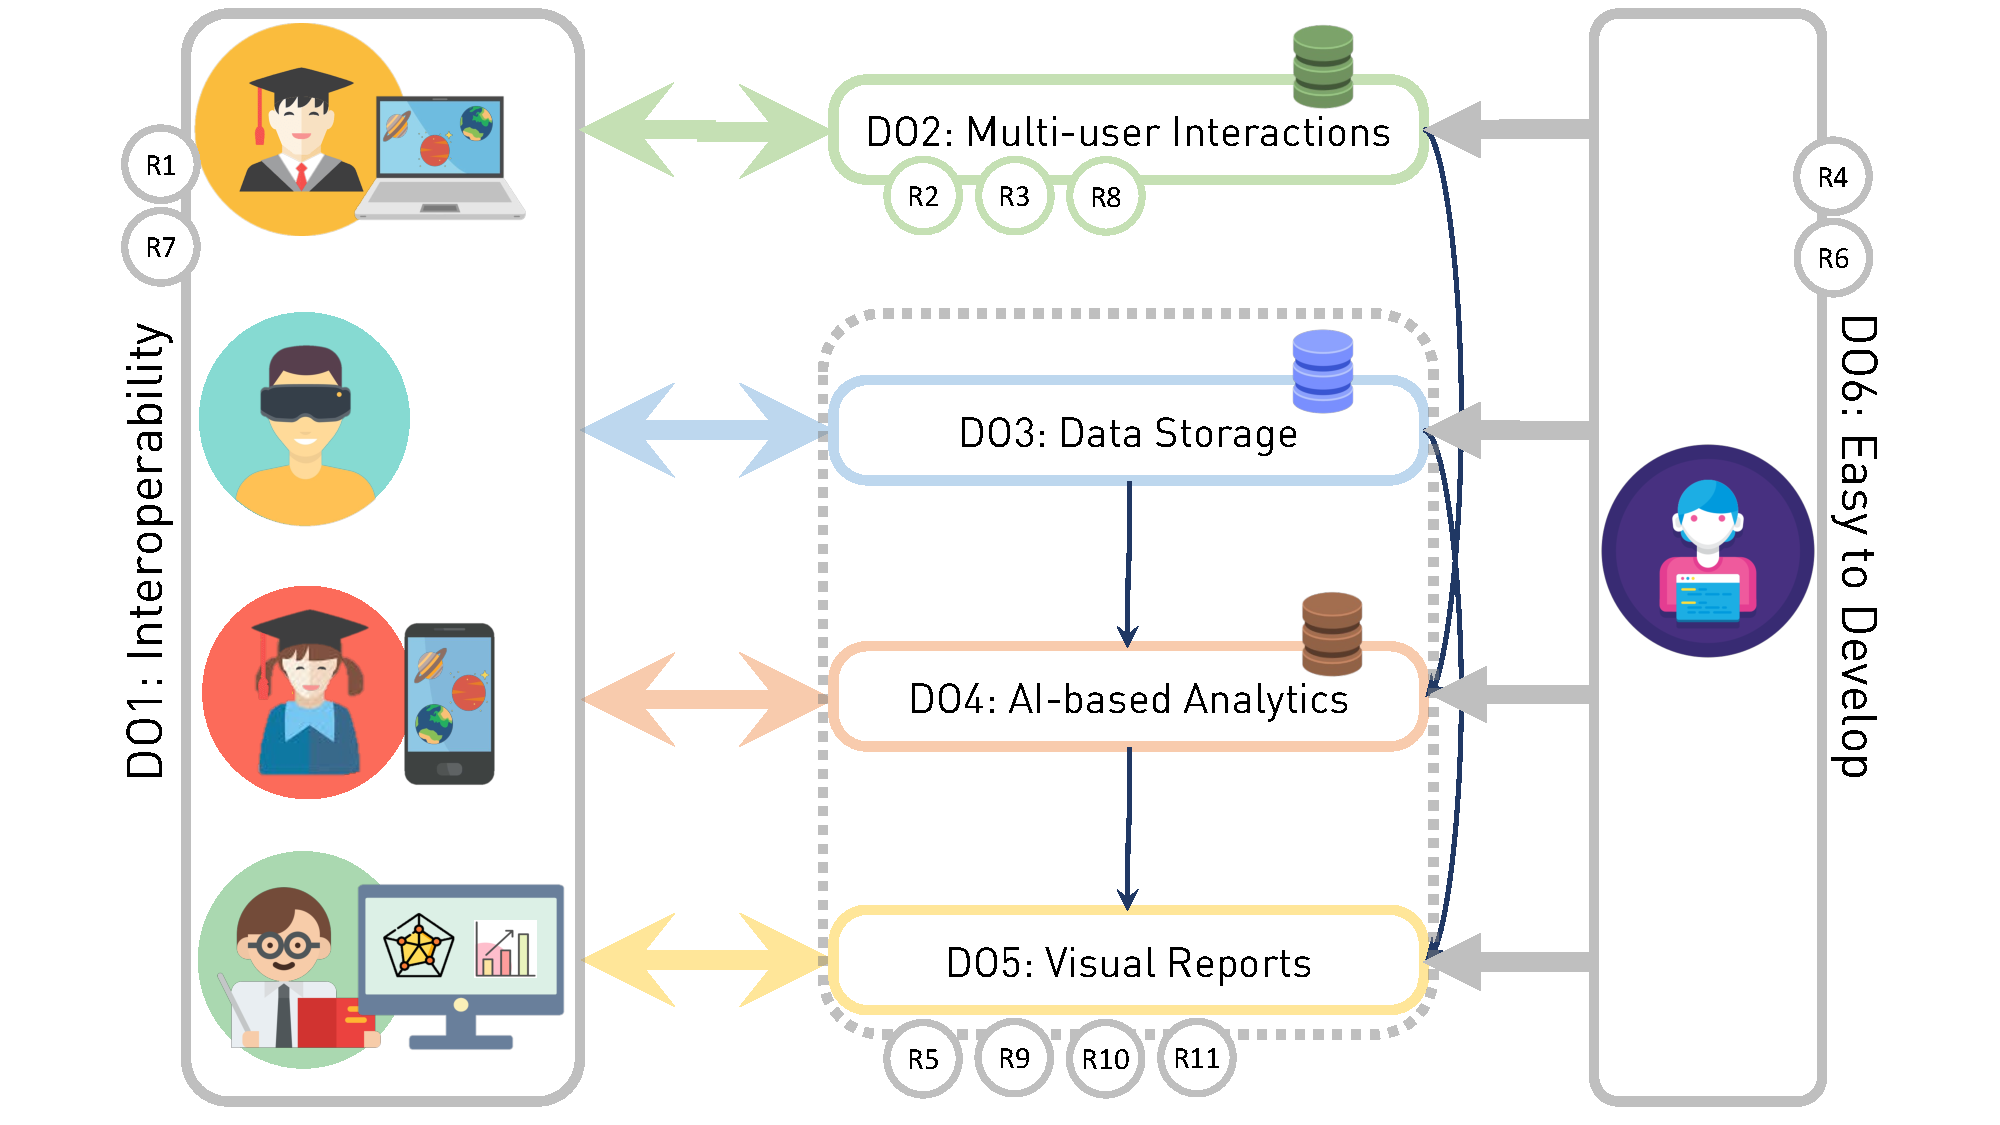
\includegraphics[width=\textwidth]{design_objs_final.pdf}
    \caption{\fontsize{10pt}{11pt}\selectfont{\itshape{A diagram representation of the architecture design objectives.}}}
    \label{fig:desobjs}
\end{figure*}

%%%%%%%%%%%%%%%%%%%%%%%%%%%%%%%%%%%%%%%%%%%%%% ARCH
\section{Architecture definition}\label{arch:architecture}

In this section \arch{} is presented. \arch{} is the architecture that fulfils all the design objectives described in Section \ref{arch:requirements}. It is a client-server architecture composed of several modules, each of which is in charge of a specific task. Two design objectives, namely interoperability (\textbf{DO1}) and ease of development (\textbf{DO6}), are not satisfied by specific modules but are rather fulfilled thanks to how the architecture has been designed. For interoperability, the definition of a web architecture and the development of multiplatform libraries ensures that developers can create applications working on different hardware (PCs, \glspl{hmd}, tablets or mobile phones) and across multiple software tools, as the architecture has been tested on multiple browsers, desktop applications as well as native iOS and Android apps. While \arch{} does not provide authoring tools that would allow AR applications to be created without requiring coding experience, extreme care was taken in developing a set of libraries and APIs that enables developers to easily create interoperable multi-user AR applications, as shown in Section \ref{arch:implementation}. 

In the following subsections, the four main blocks of the proposed architecture, summarised in Figure \ref{fig:arch}, will be described in detail. While part of the architecture has been developed from scratch, some components rely on existing libraries to provide the required functionalities. All the components have been integrated in a cohesive system that can be used to create collaborative AR applications.

\begin{figure*}[htbp]
    \centering
    %\captionsetup{justification=centering}
    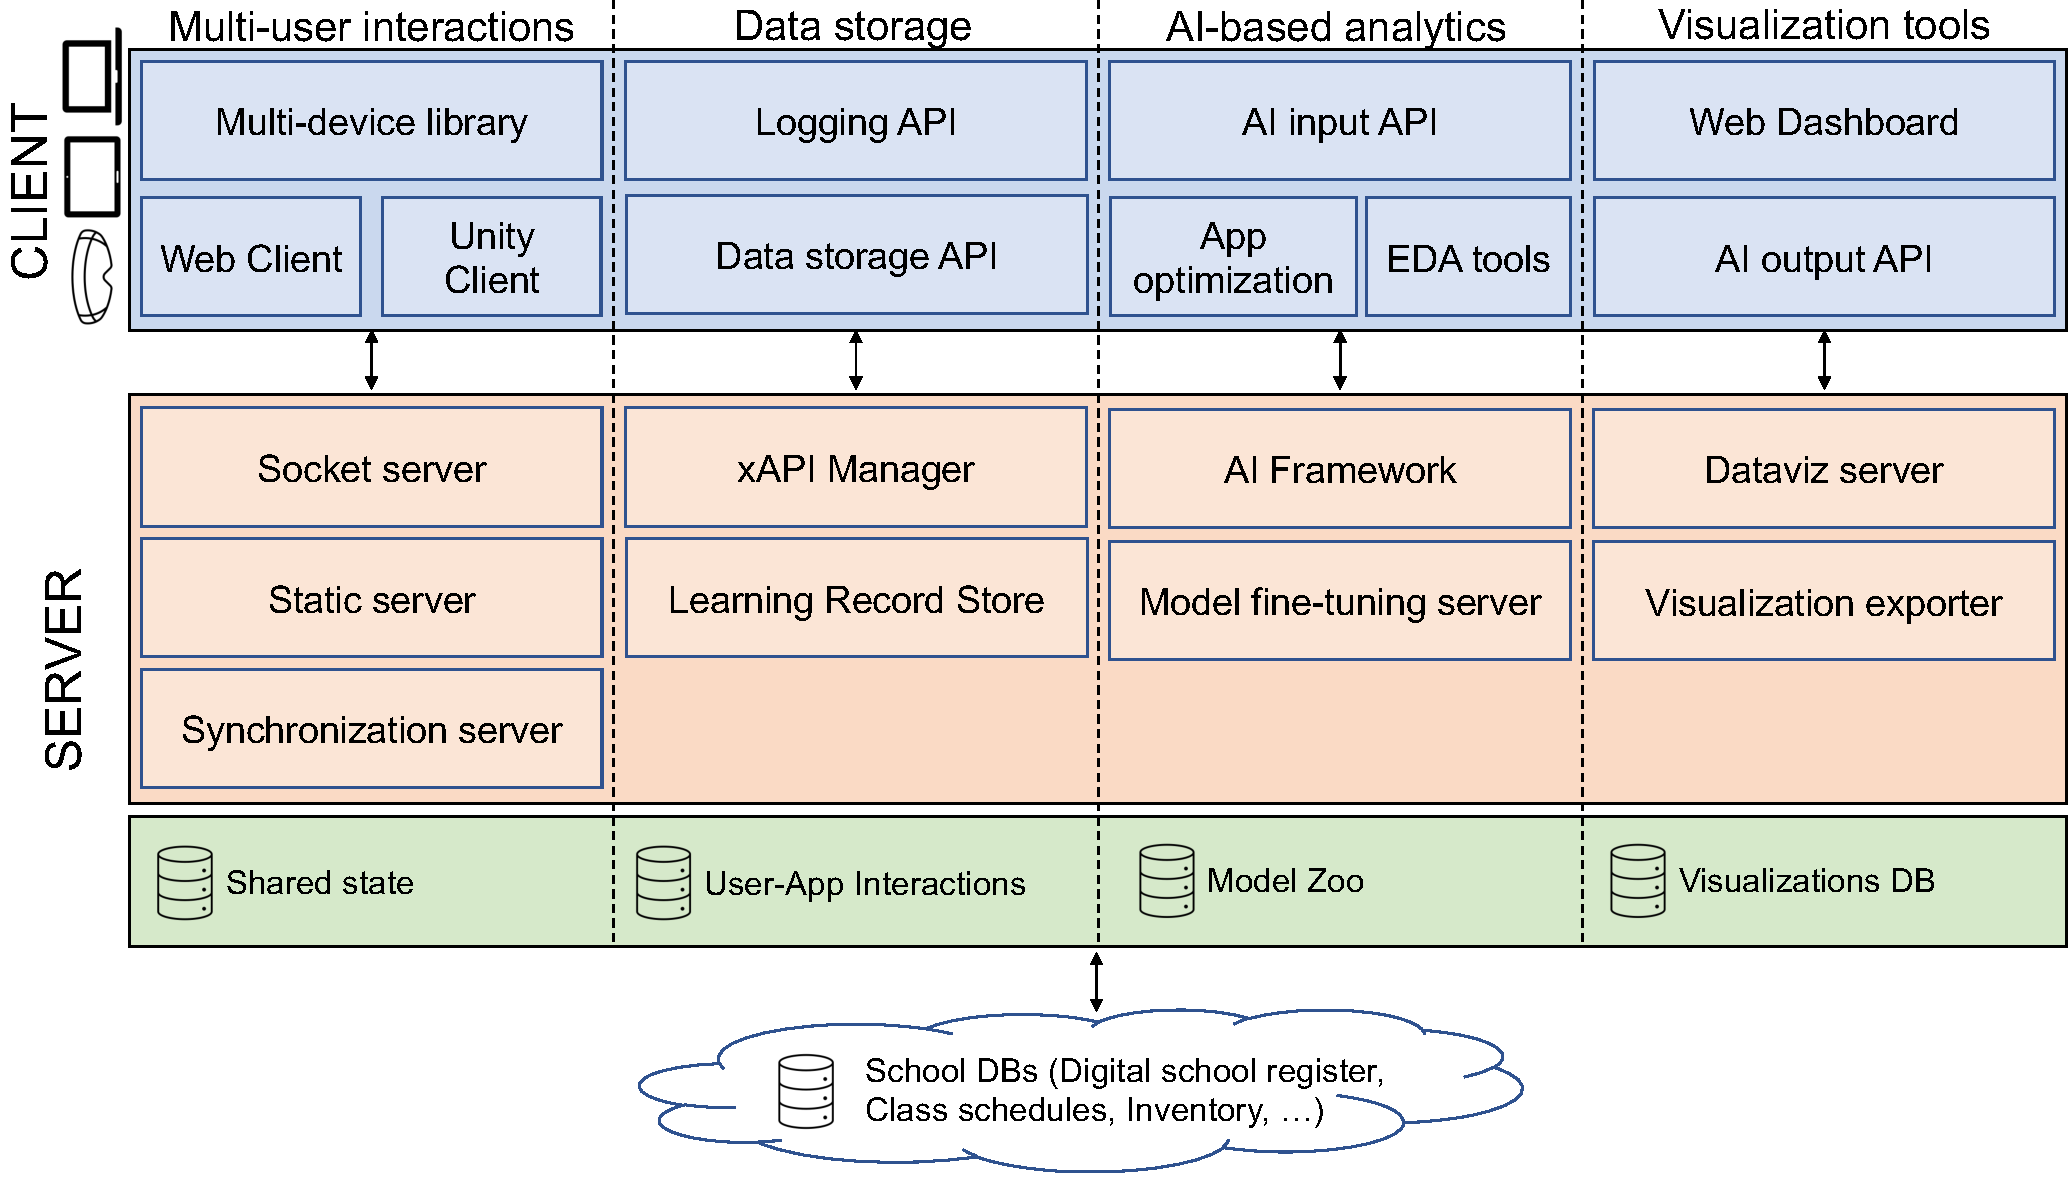
\includegraphics[width=\textwidth]{arch_diagram_revised.pdf}
    \caption{\fontsize{10pt}{11pt}\selectfont{\itshape{A visual description of the proposed architecture}}}
    \label{fig:arch}
\end{figure*}

\subsection{Mechanisms for multi-user interactions}\label{sec:architecture:multiuser}

This objective is satisfied by \ork{} \citep{10.1007/978-3-030-93907-6_106}, a library for the synchronisation and management of heterogeneous devices in multi-user applications. It is the module enabling real-time communication between multiple users. The library was initially developed in JavaScript but it also includes bindings that allow its usage in different software environments.
\ork{} simplifies the creation of multi-device applications that share state and stay in sync. To do so, the library provides functionalities such as: multi-device state synchronisation (being able to share any kind of information and have all devices in sync), video synchronisation from a centralised clock, video sharing between different devices and a service functionality where one device can publish any kind of service (e.g., authentication service) and this can be consumed by other devices.

Applications can store data of any kind and then share it with other devices. These data are the states, which will be synchronised between the different devices. When one device changes its state, it is replicated to all other connected devices.

There are two types of state:
\begin{itemize}
    \item Agent state: corresponds to the state of each device (\textit{e.g.}, the position of the device in a common reference frame relative to an AR marker).
    \item Application state: corresponds to a global state that is shared between the different devices (for example, the number of users currently connected to the application).
\end{itemize}

Through this functionality, the devices can send information to each other and keep the states synchronised. The library also allows maintaining video  synchronisation across different devices. This way it is possible to create a multi-user environment, where different users can watch the same video sequence at the same time. 

The library allows creating services between different devices so that others can consume them. For example, as shown in Figure \ref{fig:orkservices}, if a device has a model for detecting objects in images and wants other devices to be able to use such model, it can create an \ork{} service so that other devices can communicate with it and run the service.

\begin{figure*}[htbp]
    \centering
    %\captionsetup{justification=centering}
    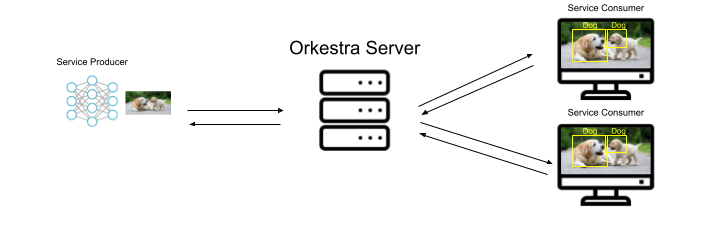
\includegraphics[width=\textwidth]{services.png}
    \caption{\fontsize{10pt}{11pt}\selectfont{\itshape{\ork{} allows creating services that can then be consumed by any devices connected to the application.}}}
    \label{fig:orkservices}
\end{figure*}

One of the main features of \ork{} is context maintenance in a multi-device environment. This is useful in multi-user applications, where all applications must have a synchronised context regardless of where they are running. The \ork{} library is in charge of:
\begin{itemize}
    \item Communication with the other devices that are also using the library and are connected to the same session.
    \item Synchronisation of the contexts with the other applications.
    \item Storage of the context of the different devices.
\end{itemize} 

In order to communicate with the other devices, the library connects to a server, which will redirect each event it receives from a device to all the other connected devices and will store the different events it receives. The context variables are stored on the server and then redirected to the other connected devices. Each client stores the context of the application and of the other devices. Each change made by a device in its context will be notified to the other devices (through the server), and they will then update their respective context.

Synchronisation of media content is achieved through the usage of a shared timeline, implemented with Motion \citep{boronat2017hybrid, montagud2018mediasync}. Motion is a service that allows multi-device applications to be synchronised from a central timer, allowing content to be adapted to a common time. It is based on the time-based multi-device synchronisation mechanism specified in the W3C draft Timing Object\footnote{\url{https://webtiming.github.io/timingobject/}}.
The service works as follows: a timing object is instantiated on each of the devices and each of these instances is connected to a single shared timeline. If one of the objects pauses, all local components are notified to act accordingly. In addition, if they are connected to the shared timeline by the server, that pause is relayed through the server to all other connected clients.
This allows synchronisation of different content according to two different types of timers:
\begin{itemize}
    \item \textit{Sequencer}: Used to synchronise content that is not media, such as different data that needs to be displayed at the same time. This can be useful in a scene-based timeline, where each scene is associated with a set of data that has to be displayed at the same time.
    \item \textit{MediaSynch}: Used to synchronise multimedia content such as video or audio. It consists of adjusting the playback speed with high precision, so that the contents are synchronised without time jumps.
\end{itemize}

\ork{} also allows connected users to send or receive video streams between all connected users. In this way, if a user wants to retransmit a video from a camera, or share a screen as a stream, they can share it via the platform and the connected users will be able to consume it. For this, the platform uses a WebRTC Janus server that is in charge of centralising the WebRTC streams, managing the sessions and forwarding the RTP/RTCP traffic between the browsers. To perform this communication with the WebRTC server by the browsers, the library provides an API that allows the user to abstain from all communication with the WebRTC server. Internally, \ork{} uses the Janus library\footnote{\url{https://janus.conf.meetecho.com/}}. This library is used in the x-media, screen-share and webrtc-publisher web components. The library also exports a method called JanusClient which uses the Janus library and allows to handle events in the communication with the WebRTC server.

Finally, \ork{} uses web components as the minimum unit of the user interface. Web components are elements that encapsulate customisable and reusable functionalities avoiding code collisions. They are based on the following principles:
\begin{itemize}
    \item \textit{Custom elements}: A set of JavaScript APIs that allow you to define custom elements and their behaviour, which can then be used as desired in the user interface.
    \item \textit{Shadow DOM}: A set of JavaScript APIs for attaching an encapsulated \textit{shadow} DOM tree to an element - which is rendered separately from the main DOM document - and controlling associated functionality. In this way, features of an element can be kept private, so it can be styled and scripted without fear of collisions with other parts of the document.
    \item \textit{HTML templates}: The template and slot elements allow you to write markup templates that are not displayed on the rendered page. These can be reused multiple times as the basis for the structure of a custom element.
\end{itemize}

%%%%%%%%%%%% OLD %%%%%%%%%%%%%%%%
% The module relies on a server for message passing between different clients and its objective is to abstract the application code from all the nuances and difficulties of network communication. While the definition of the module is platform agnostic, we recommend the usage of WebSocket \citep{rfc6455} protocol to share data across the internet with low-latency, since several frameworks support it and thus it can be integrated in any software libraries developed, for example, with Unity or any Web framework. 

% On the client side, the module defines a set of library calls enabling users to connect to a shared session, through which they can exchange messages and share data of any kind such as application variables, json files or images. On top of that, the module defines different clients enabling its usage on different platforms.

% On the server side, the module introduces synchronization mechanisms that allow clients to play multimedia tracks at the same time, enabling a shared experience, and defines a static server that keeps track of the shared state (a database defining the current state of the variables shared across users) and which is responsible for notifying any state change. Finally, the library includes a socket server which is responsible for establishing the connection with the clients and manages low-level communications.

% The library can also be used to share multimedia content, for example through the WebRTC protocol \citep{rfc7478}. In this case the module relies on another server to handle signalling and relaying data between the server and the application. The architecture is ready to work with existing solutions such as Janus or MediaSoup, which provide all the required functionalities and can be easily integrated.

% The real-time multi-user library has been designed to be simple, with the aim of reducing the latency and the time required for processing data as much as possible. Apart from the aforementioned WebSocket server and the optional WebRTC gateway, it includes a timing server to handle synchronization of the content, and a Rest API for manipulating data persistence. Connection to the server is organized via dedicated rooms, so that every user connecting to the server URI at a specific room will share the same AR experience. Rooms can be organized hierarchically and the application developers can specify the maximum amount of users per room.
%%%%%%%%%%%%%%%%%% END OLD %%%%%%%%%%%%%%%%%%%%%

\subsection{Data storage}\label{arch:architecture:logging}

Besides sharing data and messages in real time, users may be interested in permanently storing other types of data. It can be data related to the user progress in specific tasks, like the answers to a test or the completion of a chapter, or other data linked to the interactions of the user within the application, for example the number of clicks, selections in a menu, or the interactions with 3D content in the augmented space.

In this case \arch{} allows storage of data that can be serialized and stored in a database or on a local disk, and it provides means for easily querying and filtering the data when needed, either directly in the application or through a script. The architecture provides an API to store and access the data through a \gls{lrs}, thus simplifying its integration into \glspl{lms} which are already in use at school. By enabling storage of the data on an external database, applications developed with this architecture can then be integrated into the school curricula, as they can fetch data from the \gls{lms} (for example, a set of questions and answers for a test) as well as writing new data to it (\textit{e.g.}, the results of the in-app quizzes).

Finally, logging and storing usage data and activity can enable user monitoring practices. In the case of AR experiences, the teachers would be able to know how much time each student spends on different modules of an application, giving her insights on which concepts are harder to grasp. Furthermore, the teacher would be able to check if any of the students is falling behind, as the application can raise automatic flags if the student has not accessed an app in a while, or is performing consistently bad on the assessment questions. The amount of data that is stored is fully customisable at the application level, and there are options for anonymisation, adding user profiles (\textit{e.g.}, admin, teacher and student) and for changing the frequency of data collection.

\subsection{AI-based analytics}\label{arch:architecture:AI}

Given the amount of data that are made available by the module described in subsection \ref{arch:architecture:logging}, AI techniques, especially \gls{ml} algorithms, can be used to build learner and group models that can improve the learning processes. The models trained using this module are meant to be a support for the teachers, helping them gain new insights on the progress of the students or by simplifying their work, by automating some of the most time-consuming tasks.

As \arch{} is used to create AR applications, the data collected are typically of three types: \textit{natural text data}, for example all the data collected from chats or from answers to in-app questions; \textit{structured data} such as all the logs collected from the applications, organized in tables where each data point represents a student interaction; and \textit{image data}, which is data collected through interactions with the augmented content or directly from the mobile device camera. The analytics module is able to work with all these different data sources, and create models using both the supervised and unsupervised learning paradigm.

The ML algorithms are trained and stored on the server side. \arch{} allows both training of a model from scratch, or fine-tuning an existing model when new data is available. As \arch{} provides a standardised API for data input, it can work with any AI framework such as PyTorch or scikit-learn, and it supports a wide range of ML algorithms such as deep neural networks or random forests. Nonetheless, in the survey the teachers expressed the desire to understand how and why a model outputs its decisions, so the recommendation for developers is to rely on more explainable AI models \citep{KHOSRAVI2022100074} such as decision trees or linear regression models.

As the training and deployment of the models is done on the server, the client is responsible for sending the data collected to the server, and for this \arch{} provides a specific API. The client also includes tools for exploratory data analysis that allows cleaning and filtering the data in order to generate insights that can then be displayed using the visualisation module described in subsection \ref{arch:architecture:visual}. Finally, the client also includes a set of functions for the optimisation of app parameters. These functions allow, for example, the adaptation of the application to the hardware available or the network conditions, so that the developers do not have to take care of this beforehand. An example of optimisation is described in Section \ref{arch:implementation}.

Not every teacher who answered the survey was interested in applying automatic analysis of the data (and some of them were skeptical about the usefulness of it), but about 85\% of the respondents identified the most important insights the AI-based analytics module should provide. First of all, the teachers would like to retrieve information which would be hard to come by: they are interested in finding patterns in the way the students perform so that they can plan the structure of the lessons better. For example, teachers would like to have a model that, given the results to some in-app quizzes and the time when the tests were taken, predicts the time of the day the students are more focused. This could help teachers plan their daily activities.

The architecture is AI-agnostic, as it supports any algorithm \textendash{} supervised or unsupervised \textendash{} that can be implemented using standard ML libraries. An example of a model that can be created using the functionalities provided by \arch{} is a model that predicts an average score of a student on the test on a specific subject. In this case, the AR application should collect data \textendash{}which is sent in the form of \gls{xapi} statements \citep{xAPIspec} \textendash{} about how the student has been using the app. Data such as time spent on each lesson, number of interactions with the app, how quick the student was answering questions during the AR experience and so on will represent the predictor variables, while the results of the test at the end of each lesson would represent the target variables. Once the data from every student has been collected, it is then possible to train a classification model which, when given as input the predictor variables from a new student, will predict his test results on the lessons the model has been trained on.

Another category of models that is relevant for the teacher is that of unsupervised learning algorithms, especially outlier detection and clustering models. In the first case, detection of outliers can enable teachers to flag specific content (daily activity, test results or others) as outside of the standard data distribution and then decide what to do about it. In the second case, the teacher may be interested in grouping the students into different clusters, based on the metrics she consider relevant. By tracking the structure of the clusters over time, they can keep track of how the students are progressing. Finally, AI models can also help detecting which students are \textit{falling behind} and are having learning difficulties. Being able to identify these students at an early stage allows teachers to tackle the situation better and in a more effective way. In this case, the AI model will use metrics from both the logging data and the application usage data to train a classification model. As both the input data and the model parameters are stored on the server-side of the architecture, the models could be continuously improved using online model learning, while the data could even be combined to extract insights at classroom or at school level.

The tools developed in this module are not meant to replace the insights from the teachers and their experience based on daily interactions with the students. They are meant to be used as a support tool, helping teachers make decisions based on more data evidence and simplifying their work for more time-consuming tasks such as test grading.

\subsection{Visualisation tools}\label{arch:architecture:visual}

The final module provides visualisation and reporting functionalities. Through this module, the user can access a web interface where data can be displayed either as text or via interactive plots.
This module allows teachers and students, who may not have the required expertise, to visually display the data collected and to help them draw insights from it.
% Such a module is necessary because often times the teachers have neither the time nor the expertise to draw insights and conclusions from the data collected, but tools that can automatically generate plots and summaries can help them keep track of the students' progress.

%\begin{figure}[htbp]
%    \begin{center}
%    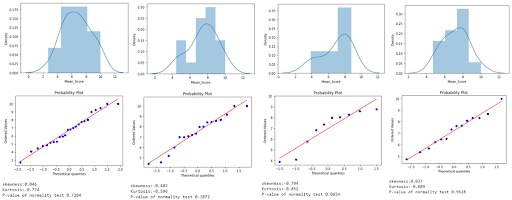
\includegraphics[width=0.94\textwidth]{viz_example.png}
%    \caption{\fontsize{10pt}{11pt}\selectfont{\itshape{An example of data visualisation created using \arch{}.}}}
%    \label{fig:dataviz}
%    \end{center}
%\end{figure}

This module relies on existing libraries for data visualisation such as D3 \citep{10.1109/TVCG.2011.185} or Seaborn \citep{Waskom2021}, but it simplifies the process of creating plots by providing an API for importing the output of the ML models, as well as a dashboard for generating interactive charts without code. %Figure \ref{fig:dataviz} shows an example of a visualisation created using data collected from xAPI statements sent from an AR application to the server.
% but it provides an API to collect the output of the existing AI models as well as a dashboards to enable displaying the plots on a browser.
The visualisations are generated on the client side. They can later be stored on the server or exported to a database, to a local storage or to the school \gls{lms}.

The visual reporting module is not meant to replace existing dataviz libraries, but rather provide teachers with a web interface that allows them to create, modify and export visualisations without requiring coding experience or directly manipulating the input data.

%%%%%%%%%%%%%%%%%%%%%%%%%%%%%%%%%%%%%%%%%%%%%% IMPL

\section{Implementation and Validation}\label{arch:implementation}

Three \gls{poc} applications based on \arch{} were created in order to validate that the software developed using this architecture satisfies the design objectives defined in Section \ref{arch:requirements}: \emph{AR Cube}, \emph{xAPI Data Analysis} and \emph{AR Geography Quiz}.

\subsection{AR Cube}

When starting the application, the users join a room and all the interactions with the virtual object are broadcast to all the users connected to the same room. The user is also able to select how often data is shared between users by selecting the time interval between the messages to the server. While simple, this application demonstrates how the architecture is able to fulfil the design objectives. The application is interoperable as it has been compiled for iOS, Android, Windows and Linux platforms and the users are able to share their AR experience when using devices running any of these operating systems. The application supports multi-user interactions in an AR environment, as the interactions with the augmented content are the same for all users. The application has been tested for up to four users, both sharing the same WIFI network and using 4G mobile connection. For the tests, two tablets (a Samsung Tab A7 SM-T500 with 3Gb of RAM and a 4\textsuperscript{th} generation iPad Air with 4Gb of RAM) and two smartphones (a Samsung Galaxy A22 5G and a Samsung Galaxy A90 5G, both with 6Gb of RAM and running on Android 11) were used. The average latency (measured as the time spent since the request is sent from a user to the instant when it is received by all users) was 205 milliseconds. There was no appreciable difference in latency between WiFi and cellular network, but for messages sent from a mobile phone the latency was significantly lower than the one measured for messages sent from a tablet (mean value of 96 ms vs. 245 ms). For this PoC, the latency value was not affected by the number of clients connected or the amount of messages exchanged by the end users. For more complex applications, the resources allocated in the backend should be properly tuned in order to guarantee the desired latency.

\begin{figure}[htbp]
    \begin{center}
    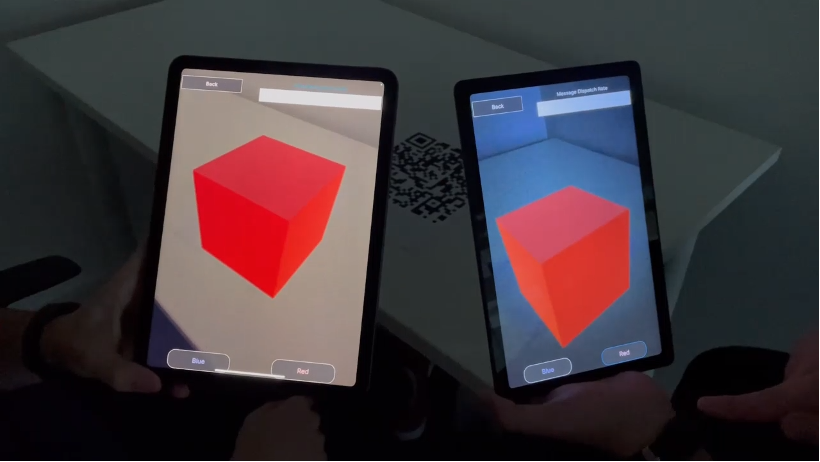
\includegraphics[width=0.94\textwidth]{AR_cube.png}
    \caption{\fontsize{10pt}{11pt}\selectfont{\itshape{The AR Cube PoC accessed by two users sharing the same AR marker.\protect\footnotemark}}}
    \label{fig:arcube}
    \end{center}
\end{figure}

\footnotetext{A video demo is available at \url{https://anon.to/pwRr4W}}

One of the parameters of the application is what is called the \emph{dispatch time}, which is the time interval between two consecutive messages from the same user. For interactions generating many events (such as the rotations of the cube when swiping the screen), the user could generate up to 30 events per second. To prevent the application from slowing down (or even to saturate the network, for more data intensive applications), events are stored in a queue and then sent together once the dispatch time has elapsed. This way, it is possible to find a balance between the smoothness of the rotation and the amount of events sent. When a reasonable dispatch time value was selected (from 0.01 to 0.04 seconds), every user was able to experience a very smooth cube rotation. The dispatch time could also be set automatically by the application: if the user does not select a value, the app estimates the latency (by measuring the time elapsed between sending a message and receiving it back) and modifies the dispatch time accordingly until the desired latency value is achieved. 

Finally, the PoC shows how easy it is to develop for \arch{}. The object model properties, the application logic and the integration with the library for multi-device access required less than 400 lines of code. To enable multi-user interactions in the application, the developers only needs to register the events that affect all the users (the rotations and the color changes, in this PoC), to add a call to the function that generates a notification for these events, and to create a subscriber object which receives the notifications and modifies the app context which will then propagate the information to every user.

\subsection{xAPI Data Analysis}
The second PoC features a \gls{lrs} that collects data from users accessing a web page (Figure \ref{fig:xapi_generator} shows the UI of the app). The application keep tracks of both active interactions (mouse clicks, text entered, etc.) as well as passive ones such as time spent on the page or date of access. The data is collected in the form of statements which use a vocabulary specifically created for the demo application. The server side uses Learning Locker, and all statements are stored in a MongoDB\footnote{\url{https://www.mongodb.com/}}. This PoC simulates the process of data collection that could be performed in a generic AR application, and was built to test the integration of \arch{} with Learning Locker\footnote{\url{https://learninglocker.atlassian.net/wiki/spaces/DOCS/overview}} and scikit-learn, as well as the ability of the architecture to handle huge volumes of data without appreciable delay. Learning Locker is the standard data repository for storing learning activity statements generated by \gls{xapi}.
\gls{xapi} is a web service that enables the secure sending and storing of learning experiences to an \gls{lrs}.
\gls{xapi} statements use JSON format and at their core they are formed by the triplet \textit{Actor--Verb--Object}.
The \textit{Actor} represents the person performing a specific action (the \textit{Verb}), while the \textit{Object} could be another person or an xAPI activity on which the actor acts upon.
xAPI statements can optionally include additional information such as \textit{Timestamps}, \textit{Context} or \textit{Results}, to provide more detailed information. Apart from the client interface for the user, another web page allows the statements to be downloaded, possibly applying different kind of filters, in a JSON format for further processing. Furthermore, a script performs weekly incremental backups of the database, copying the statements from the AWS instance where the LRS is running to a local storage.

\begin{figure}[ht!]
    \begin{center}
    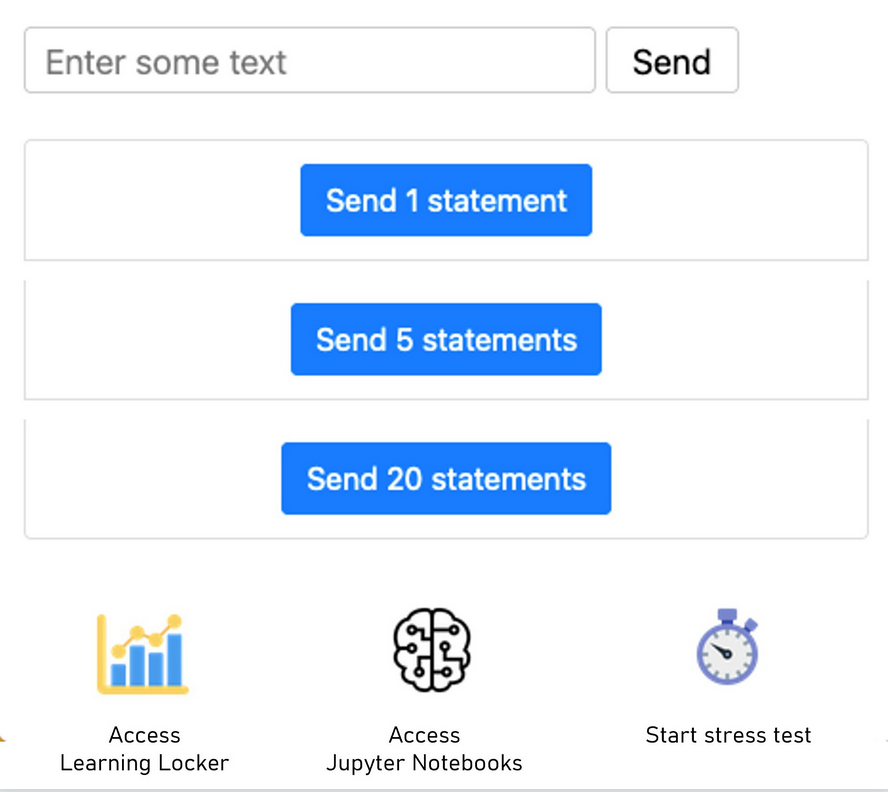
\includegraphics[width=0.6\textwidth]{xAPI_generator_v2.png}
    \caption{\fontsize{10pt}{11pt}\selectfont{\itshape{The user interface of the xAPI Data Analysis PoC. Statements are generated manually or automatically, by starting a stress test or by tracking user activity. Additional UI elements allow accessing the Learning Locker where the statements are stored as well as the notebooks used to create the AI models.}}}
    \label{fig:xapi_generator}
    \end{center}
\end{figure}

Learning Locker provides an interface for filtering the data and for the creation of dashboards for data visualisation. This way, a user can explore and visualise information without having to write a single line of code. Besides the tools offered by Learning Locker, a set of functions for data cleaning, data exploration, data modelling and data visualisation were developed. These functions allow more experienced users to get more insights than the ones provided by Learning Locker and to run classification, predictive and clustering algorithms. Even though the code has to be modified and adapted for each application, using xAPI as a data format allows the creation of a standard set of library calls that favours data reuse.

To measure the ability of the deployed solution to handle the processing and storage of xAPI statements, a stress test was performed where 10 clients were generating multiple statements per seconds. A short summary of the testing conditions is available in Table \ref{tab:xapistress}. During the test, the clients sent close to 80000 statements to the LRS. The average delay between the sending of a statement and its availability on the LRS was 145 ms, with a maximum delay of 314 ms. 

The statements generated during the stress test were also used as training data to create a simple ML classification model. The data storage and AI analytics modules of the architecture were used to fetch the data and perform the preprocessing step, which parses the data stored as JSON to extract the relevant input features. The independent variables used to train the model are extracted from the triplet \textless actor, verb, object\textgreater{} associated with each xAPI statement, as well as additional information such as the time delay between consecutive statements. The only statements used to train the model were the ones using \textit{sample} as their verb, and a typical statement would be for example \textless \emph{client-01}, \textit{sample}, \emph{1.04}\textgreater{}. The object value for these statements is a number sampled from a gaussian distribution whose mean and variance depend on the client that generated it. The statements were preprocessed to obtain a two-column input matrix \textendash{} \emph{ID} and \emph{sample} \textendash{} which could be fed to a linear classifier. Later, at test time, the model was able to successfully predict which client generated a specific statement, based on the value passed in the object of the statement triplet.
%The model learned then to predict the client that originated a particular statement.

\begin{table}[ht]\centering
%\renewcommand{\arraystretch}{1.1}
\caption{\fontsize{10pt}{11pt}\selectfont{\itshape{xAPI statements sent during the stress test of the second Proof  of Concept app.}}}
\begin{tabular}{cccc}
\toprule
Test & Statements/batch & Wait time & Statements \\
\midrule
1 & 15 & 10s & \textbf{1653} \\
2 & 30 & 5s & \textbf{6614} \\
3 & 30 & 2s & \textbf{16534} \\
4 & 50 & 1s & \textbf{55116} \\
\midrule
Total & & & \textbf{79917} \\
\bottomrule
\end{tabular}
\label{tab:xapistress}
\end{table}

\subsection{AR Geography Quiz}
The last PoC implemented is a more complex AR application that simulates an interactive geography quiz which, for example, could be used in a classroom to evaluate the knowledge of the students regarding subjects they recently studied (see Figure \ref{fig:argeo} for an example of what the teacher interface looks like). 

\begin{figure}[!ht]
    \begin{center}
    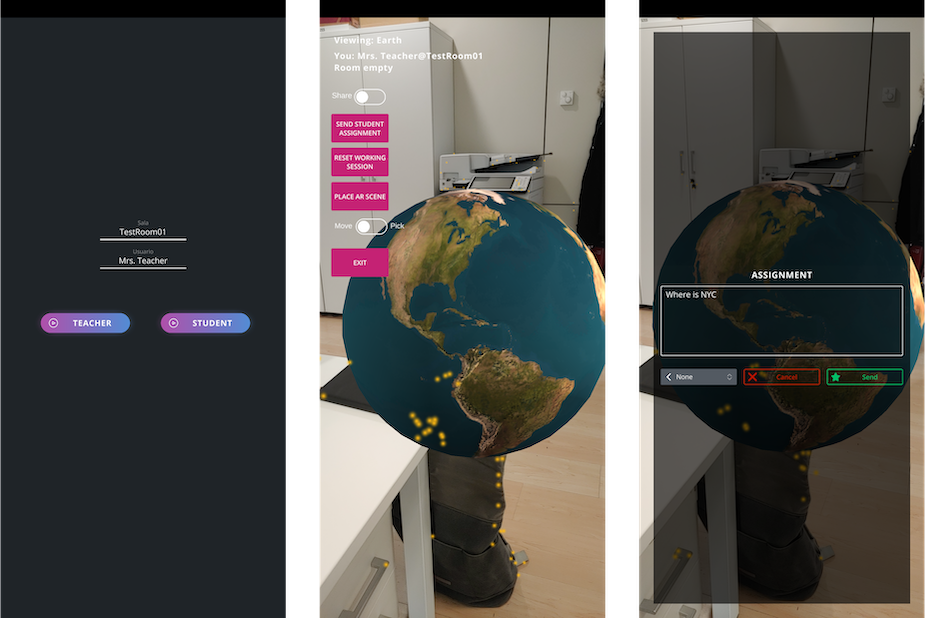
\includegraphics[width=0.9\textwidth]{PicGeoAR.png}
    \caption{\fontsize{10pt}{11pt}\selectfont{\itshape{The AR Geography Quiz application. From left to right: the login screen, the augmented content, the ``send question'' view.\protect\footnotemark}
    \label{fig:argeo}}}
    \end{center}
\end{figure}

\footnotetext{A video demo is available at \url{https://anon.to/4Ulhto} \label{argeofn}}
 
In this example, AR Foundation was used to create an AR scene in Unity where the user sees a 3D model of the Earth and she can change what she sees by swiping the finger on the display or by physically moving around the 3D element. In the application, one teacher and one or more students connect to the same virtual room to participate in the quiz (the video linked in \cref{argeofn} only shows interactions between the teacher and one student, for the sake of simplicity, but the PoC also supports one-to-many interactions). The application works in two modalities. In the first one, each user can freely explore the augmented content, either by rotating the globe or by actually moving around it, and there is no shared experience between users. In the second modality, one user can force every other user to watch the globe from their perspective, and it is in this modality that the users are sharing their interactions. For example, the teacher has the ability to force every user to see the 3D Earth from his \gls{pov}, forcing the AR camera position to be the same for all users, and to send questions such as \textit{Where is Canada?} to a specific user. When that happens, the student who received the question will then share their camera PoV (effectively controlling what other users are seeing on their device) and he can answer the question by placing a marker on the globe. Once that is done the teacher will re-gain control of the application and mark whether the student answered correctly. A multi-user AR application for education can make the learning experience more engaging and promote collaboration between users by enabling interactions with the environment and also with other students.

This PoC , like the first one, uses \ork{} for multi-user interactions management, and it has been compiled for both desktop and mobile (Android and iOS) platforms. A server is used to store and forward all the events and messages passed between the clients, and an online database is used to store the questions, answers and the progress of each student.


%%%%%%%%%%%%%%%%%%%%%%%%%%%%%%%%%%%%%%%%%%%%%%

\section{Final remarks}\label{arch:conclusions}

In this Chapter \arch{}, an architecture enabling the creation of interactive and collaborative AR applications for education, was presented. To define the design objectives of \arch{}, a survey of the existing literature on the subject was performed. Then, the architecture requirements were gathered from a survey completed by primary and secondary school teachers. \arch{} is composed of four different modules, responsible for enabling multi-user interactions, data storage, data analytics and visualisation. Three demo applications were created to demonstrate that the architecture complies with the design objectives. \arch{} will help developers in the creation of AR applications that could be easily included in existing school curricula. This in turn will provide the teachers with a suite of tools that enables them to keep records of student activity, add smart analytics and automatically create reports about student progress and retention. 

\begin{table*}[htb]\centering
\caption{\fontsize{10pt}{11pt}\selectfont{\itshape{Summary of design objectives fulfilled by each proof of concept application.}}}
\resizebox{\textwidth}{!}{
\begin{tabular}{cccccc}
\toprule
     & \multicolumn{5}{c}{\textbf{Design Objective}} \\ 
\cmidrule(lr){2-6}
& \multicolumn{1}{c}{Interoperability}  & Multi-user & Data Storage & AI support & Easy to develop \\
\multicolumn{1}{c}{\textbf{Proof of Concept}} & DO1 & DO2 & DO3 & DO4 & DO6 \\
\midrule
\multicolumn{1}{c}{AR Cube} & \checkmark & \checkmark & & \checkmark & \checkmark \\ 
\multicolumn{1}{c}{xAPI Data Analysis} & & \checkmark & \checkmark & \checkmark & \checkmark \\ 
\multicolumn{1}{c}{AR Geography Quiz} & \checkmark & \checkmark & \checkmark & & \\ 
\bottomrule
\end{tabular}}
\label{tab:summarypoc}
\end{table*}

The \glspl{poc} developed demonstrate how \arch{} fulfils the design objectives identified in both the literature and the conducted survey. Table \ref{tab:summarypoc} summarises which design objectives are satisfied by each PoC. AR Cube is clearly interoperable, as it has been tested on several operating systems. It also shows that multi-user capabilities can be easily integrated into any application. This PoC also implements an AI-based algorithm that automatically sets the value of the \textit{dispatch time} based on the current network conditions. The xAPI Data Analysis \gls{poc} is a web-based application which allows multiple users to interact and stores the interaction statements in a learning record repository. Enabling storage of xAPI statements is straightforward, and AI support is guaranteed by the implementation of classification models which use the data gathered from the recorded statements as input features. The last PoC, AR Geography Quiz, is more complex than the first two PoCs. It has been developed for both web and mobile platforms and is inherently multi-user. It also demonstrates that \arch{} enables data storage in the developed applications as all the interactions, as well as the questions and answers, are stored.

% \begin{table*}[ht]\centering
% %\renewcommand{\arraystretch}{1.3}
% \caption{\fontsize{10pt}{11pt}\selectfont{\itshape{Summary of design objectives fulfilled by each proof of concept application.}}}
% \resizebox{\textwidth}{!}{
% \begin{tabular}{cccccc}
% \toprule
% \diagbox{Proof of Concept}{\textbf{Design obj.}} & Interoperability & Multi-user & AI support & Data Storage & Easy to develop \\

% \midrule
% AR Cube & \checkmark & \checkmark & \checkmark & & \checkmark \\
% xAPI Data Analysis & & \checkmark & \checkmark & \checkmark & \checkmark \\
% AR Geography Quiz & \checkmark & \checkmark & & \checkmark & \\
% \bottomrule
% \end{tabular}}
% \label{tab:summarypoc}
% \end{table*}

The architecture presented can work with most of the software suites currently in use to produce AR applications. Since it is modular, developers can choose which parts of the architecture should be integrated into existing applications. As the majority of existing AR apps are client only, the most critical aspect for integration with existing software is the provision of a server which provides all the desired functionalities. It is recommended at first to integrate the data storage and visualisation modules, and only later add multi-user and AI functionalities.

\chapter{Validation of the Proposed Architecture}
\chaptermark{Validation}
\label{chap:eval}

This Chapter presents an application called \appname{}, a multiplatform AR application for education. It is based on the \arch{} architecture presented in the previous chapter, and designed with the help of secondary school teachers. The app provides interoperability, multi-user support, integration with LMSs and data analytics capabilities, thus simplifying the development of collaborative AR learning experiences. \appname{} was developed with the purpose of validating, in an educational environment, the \arch{} architecture.
The application has been tested by \numstudents/ students and 3 teachers from \numschools/ different educational institutions to evaluate the usability as well as the impact of collaboration functionalities in the engagement of the students.

%%%%%%%%%%%%%%%%%%%% INTRO %%%%%%%%%%%%%%%%%%%%%%%%%%
\section{Overview}\label{eval:introduction}

In the last few years, significant improvements in both hardware and software have led to a proliferation of AR applications for mobile devices and AR headsets, and extensive research has been conducted on the integration of AR in education \citep{7943075, akccayir2017advantages, chen2017new, ibanez2018augmented, pellas2019augmenting, 10.3897/jucs.76535}. However, despite these advancements and research efforts, the use of AR in primary and secondary schools is still not common \citep{doi/10.2759/121671}.
The main reasons behind this were identified in Chapters \ref{chap:sota} and \ref{chap:arch}, namely the limited collaboration capabilities of existing apps, the inability to create new content and the difficulty of adapting to existing school curricula.
In Chapter \ref{chap:arch}, \arch{} was presented as an interoperable architecture. It enables the creation of multi-user AR applications and simplifies the development process. \arch{} also allows the stakeholders to add new content to existing applications, track user progress and integrate application data into the \gls{lms} used by the teachers.

The analysis of the answers provided by the teachers allowed the identification of 6 \glspl{do}, as described in Section \ref{arch:architecture}. A conceptual evaluation of the \arch{} architecture was performed through the creation of 3 \glspl{poc} (presented in Section \ref{arch:implementation}). The aim of this initial evaluation was to demonstrate that \arch{} fulfils the aforementioned \glspl{do}.

% \begin{itemize}
%  \item \textbf{Interoperability (DO1)}: The architecture enables the creation of applications that can run on multiple devices \textendash{} tablets, smartphones, \glspl{hmd} or laptops \textendash{} and provide APIs for development on multiple platforms.
%  \item \textbf{Multi-user capabilities (DO2)}: As collaboration is a key requirement, the architecture provides tools to support multi-user functionalities, both for remote and in-class collaboration.
%  \item \textbf{Data analytics (DO3)}: The architecture enables long-term data storage as well as tools for automatic data analysis and visualization, by providing an API to access standard dataviz and machine learning libraries.
%  \item \textbf{Easy to develop (DO4)}: The applications relying on the architecture can be developed quickly and easily.
%  \end{itemize}
 
% In the previous Chapter, three \glspl{poc} were described. Their aim is to perform a conceptual evaluation of the architecture and to demonstrate that it fulfills the aforementioned \glspl{do}.

This new Chapter builds upon such previous work and introduces \appname{}, a multiplatform collaborative AR geography game.
The primary goal of the application is to demonstrate the potential of the \arch{} architecture for creating interoperable applications that can be integrated into school curricula\footnote{The application is open source and the code can be accessed at \url{https://github.com/tv-vicomtech/ARoundtheworld}}.
Additionally, the game aims to enhance student engagement through the collaborative functionalities provided by \arch{}.
%how collaborative \gls{ar} applications built using the cleAR architecture can increase students' engagement and be easily included in school curricula, thanks to its integration and customisation capabilities.
The application has been developed incorporating feedback from the teachers of a Basque primary and secondary school association\footnote{\url{https://ikastola.eus/}} and it has been evaluated after being tested with \numstudents/ students in three different educational institutions.
Once the test was complete, teachers were interviewed while students were asked to fill in a short questionnaire about the \appname{} \gls{ui} and the \gls{ux} it offered. The questionnaire also asked about the app effectiveness as a tool for raising the engagement of the students and enabling collaboration between them.
To perform a quantitative evaluation about \appname{} collaboration capabilities, the app collected data \textendash{} in the form of xAPI statements \citep{xAPIspec} \textendash{} about its usage, the number of interactions between students and their performance.

The choice of Geography as the application domain is motivated by the fact that geographical exploration is an integral part of child development \citep{catling1993whole}, and the use of maps helps students improve spatial thinking skills \citep{collins2018impact}.
The application is structured as a quiz where students take turns to answer Geography questions.
If a student is struggling to answer a question, other students can interact in the augmented space and provide hints to the active user.
\appname{} works both as a mobile and a web application, is easily extensible and provides several logging and tracking mechanisms, which can be easily integrated into the \gls{lms} of the school to enable automatic tracking of the progress of the students.

The main contributions of this Chapter can be summarised as:
\begin{itemize}
    \item A complete description of the application and the feasibility of implementing the different components of the \arch{} architecture to fulfil all the design objectives;
    \item A qualitative evaluation of the technology integrated in the application, based on the questionnaires filled in by the \numstudents/ students and the interviews with their teachers;
    \item An analysis of the data collected by the application during the user study, with a focus on the effects of collaboration capabilities on the quiz results and the engagement of the students.
\end{itemize}

The number of users who participated in the study is not representative of the whole student population. The aim, in this case, is not to demonstrate the positive effects of AR in schools, but rather to validate the architecture presented in a real educational setting, and not only through the development of PoCs.

The rest of the Chapter is structured as follows: Section \ref{eval:related} covers the relevant state of the art.
Section \ref{eval:appdesc} describes the implementation details of \appname{}, while Section \ref{eval:evaluation} outlines our methodological framework and the evaluation process.
In Section \ref{eval:results}, the results obtained from the student questionnaires and teacher interviews are described, together with the quantitative analysis of the data collected through the application.
Finally, Section \ref{eval:conclusion} presents some final remarks. 

%%%%%%%%%%%%%%%%%%%% RELATED %%%%%%%%%%%%%%%%%%%%%%%%
\section{Related Work}\label{eval:related}

A recent review of AR applications used in education \citep{eleniiattro} mentions that collaborative learning in AR represents a critical research direction, but so far very few studies provide collaborative functionalities in an AR environment \citep{9645428, choi2017arclassnote}.
The work from \cite{cai2017applications} presents an application that makes use of a Kinect camera to extract 3D information from the scene and display virtual magnetic induction lines.
In \citep{takahashi2018empathic}, the authors designed a large scale AR and projection system, modifying the gymnasium of the school, to create a learning game for children with \gls{asd}, which was designed to keep their attention focused on the content provided.
\cite{laviole2018nectar} presented a markerless application for learning how an artificial neural network works, where the students can manually tweak the values of the network parameters and see how it affects the ability of the network to classify images.

As it heavily relies on visual representation of data, several technologies have been exploited to make the teaching of Geography more effective and engaging.
In the context of AR, \cite{palaigeorgiou2018touching} used a projector to create tangible 3D maps with which up to three students could interact at the same time.
\cite{xefteris2019mixing} extended the concept of tangible maps by including the usage of programmable robots to guide the students through a virtual journey. A collaborative AR app for teaching geography and geology is the one presented in \citep{wellmann2022open}. The app relies on a AR sandbox\footnote{\url{https://ar-sandbox.eu/}} to display the content and it allows teacher to modify its behaviour by writing code in the form of Jupyter notebooks.

As far as evaluating the effectiveness of AR applications for education, the vast majority of the studies highlight a positive (albeit limited) effect derived from using the technology.
\cite{CHANG2022104641} performed a meta-analysis of 134 studies which suggests that AR benefits all the learning outcomes evaluated, with the largest effect being on students performance.
A systematic review of 45 studies \citep{da2019perspectives} reaches the same conclusions, but highlights the many differences in the evaluation protocols, which complicate the statistical analysis of AR effectiveness across different applications.

AR applications are often implemented as serious games, in which using gamification concepts the students can more easily learn and retain concepts that would otherwise not interest them.
\cite{oh2017hybrid} described a game-based simulation where the users can study the properties of light such as reflection and refraction.
\cite{lopez2020emofindar} created a multiplayer game in which children can improve their communication skills by practicing in an AR environment, while \cite{ccelik2022use} described a gamified AR app used in a Content and Language Integrated class.

Several publications focus on the importance of effective \glspl{ui} and \glspl{ux} in enhancing student engagement.
A systematic review of the literature analysed 49 studies \citep{LAW2021100321} and identified a lack of information about usability and user experience frameworks, suggesting that there is a disconnect between Human-Computer Interaction (HCI) and \gls{tel} communities, as well as a lack of AR-specific \gls{ux} evaluation metrics.
The work of \cite{thamrongrat2019design} evaluated the learning effect for teaching 3D geometry using an AR application compared to traditional learning, as well as the user engagement of the students using the app compared to the ones in the control group.
Another study \citep{alrashidi2017evaluating} compared the effectiveness of learning software debugging concepts using an AR application versus a non-AR approach.

Applications used in schools usually generate data that are stored on the school \gls{lms}.
A standard that is recently gaining traction for collecting data about the activities of the learners is eXperience API, an open-source software specification that makes it possible to collect data about a wide range of learning experiences. This is achieved by sending each activity that needs to be recorded to a \gls{lrs} in a consistent and secure format \citep{xAPIspec}.
The activities are collected as statements stored as JSON objects.
Statements can be tuned to a specific use case by defining a vocabulary of valid statements.
\cite{9225931} described a system where xAPI is used to perform learning analytics in an AR environment, while \cite{wu2020design} used xAPI to collect data for a 3D design course.

%%%%%%%%%%%%%%%%%%%% APP DESC %%%%%%%%%%%%%%%%%%%%%%%
\section{Collaborative AR application}\label{eval:appdesc}

This Section describes how the application is implemented and how the developed application fulfils the \gls{do}s presented in Section \ref{arch:req:desobj}.
The application, called \appname{}, is a collaborative geography quiz in which students answer a set of questions prepared by the teacher.
Once started, the application sends a question to the first student (for example, \textit{Where is Kyoto?}). The student answers by placing a pin on the 3D globe of the Earth shown in the augmented space.
Other students can collaborate with the active user in two ways. They can suggest to her in which continent the answer is located and \textendash{} once the user has placed the pin but has not confirmed her choice yet \textendash{} by sending a \textit{thumbs up} or \textit{thumbs down} feedback\footnote{A video description of the application is available at this link: \url{https://anon.to/a7NPy8}}.
Once a student answers, the application sends a new question to the next user, and repeats the process until all the questions have been answered.
Figure \ref{fig:app_workflow} shows the application workflow, highlighting the interactions of teacher and students.

\begin{figure*}[htbp]
    \centering
    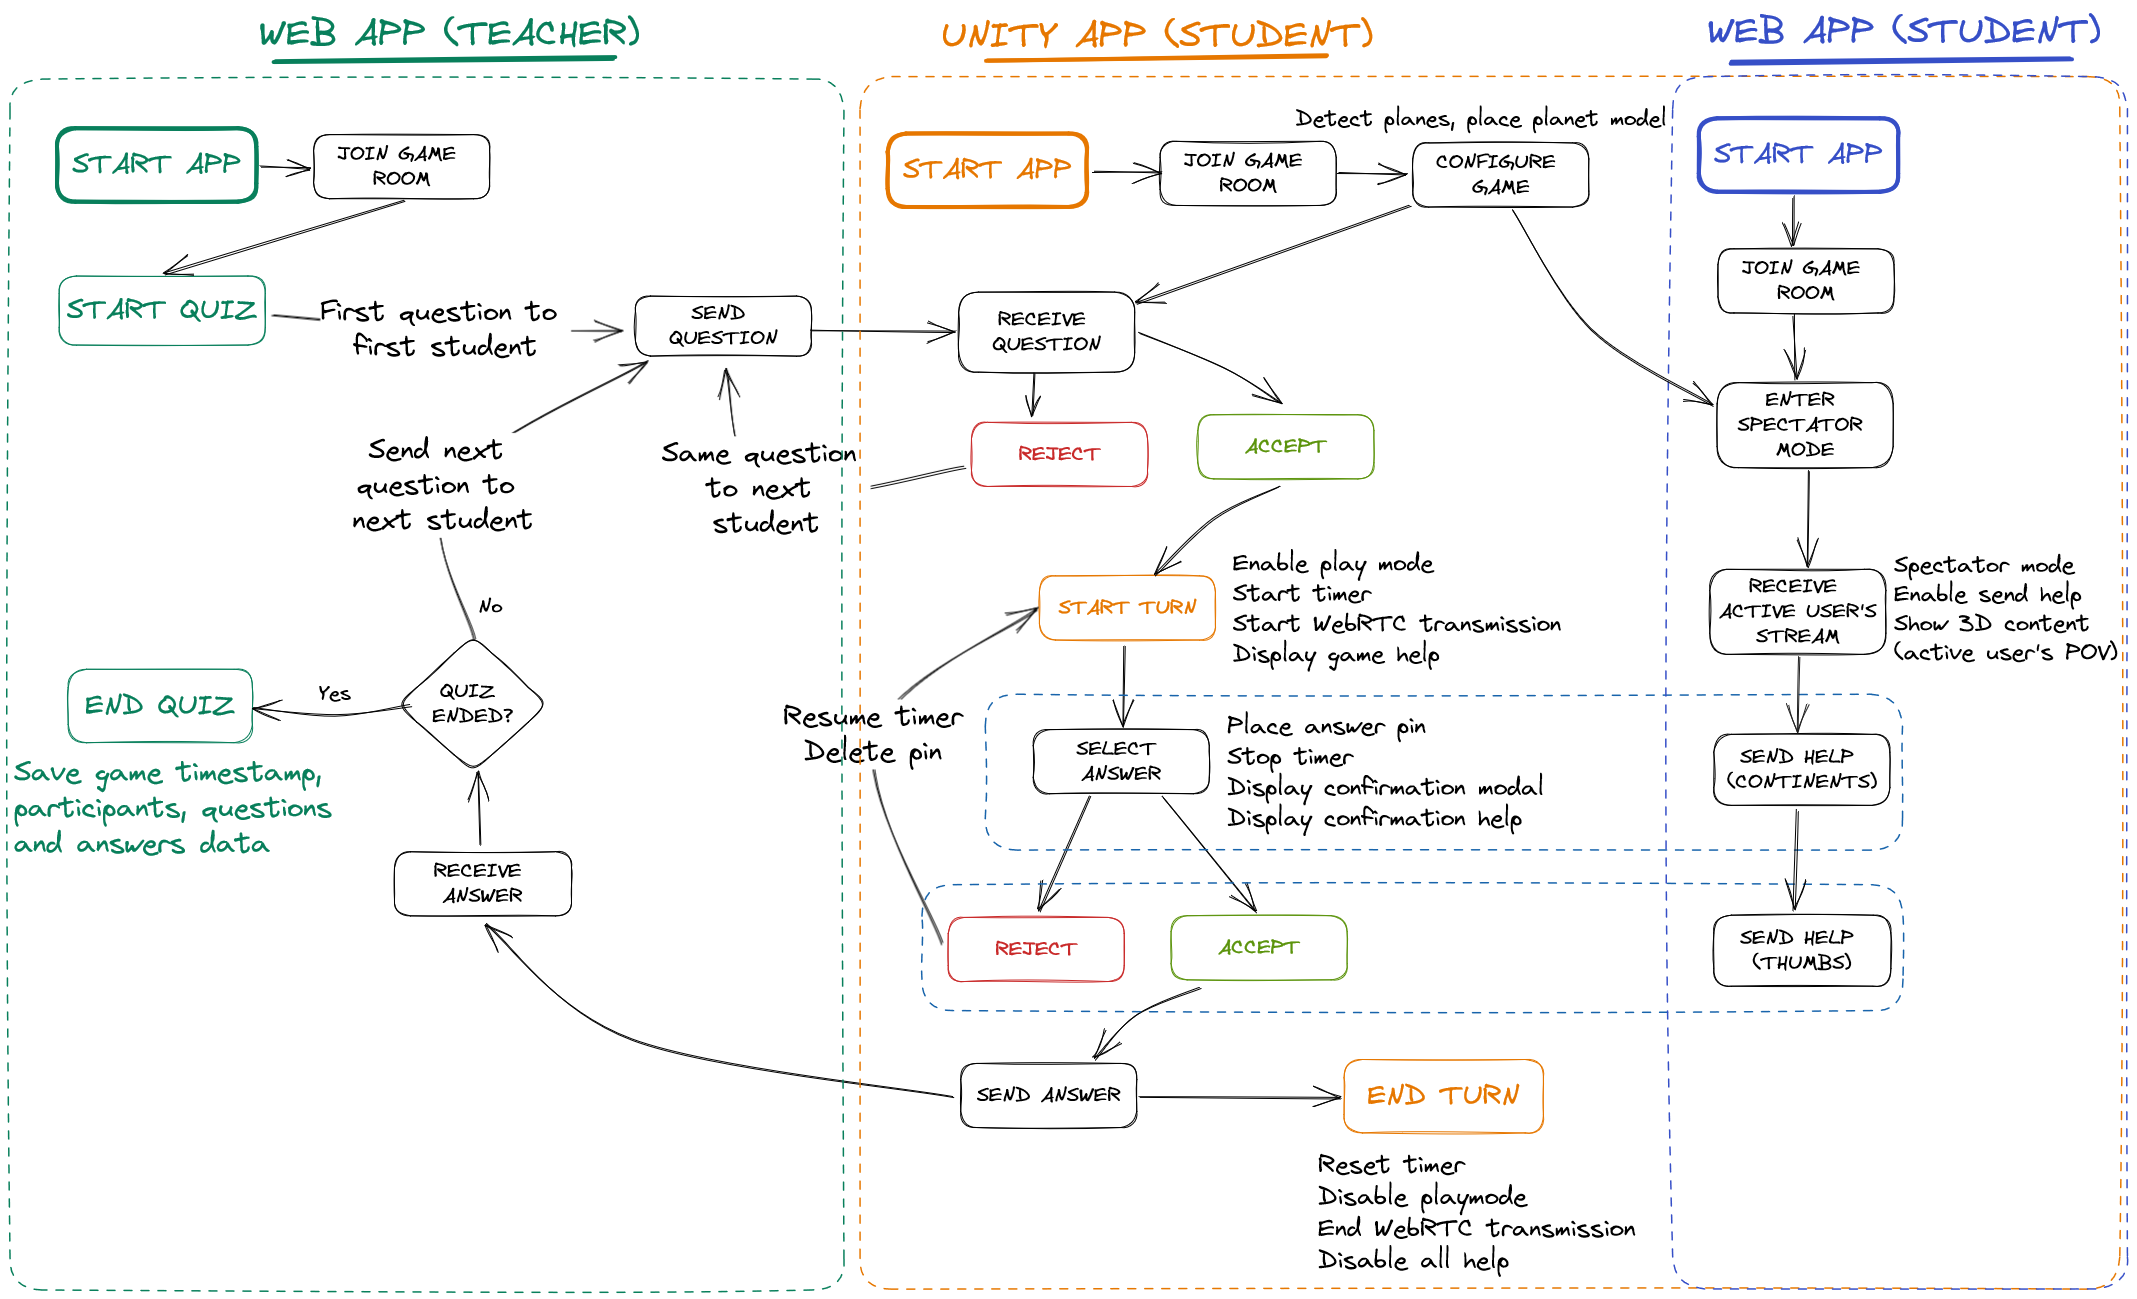
\includegraphics[width=0.95\textwidth]{workflow_diagram_3.png}
    \caption{\fontsize{10pt}{11pt}\selectfont{\itshape{Workflow of the \appname{} application.}}}
    \label{fig:app_workflow}
\end{figure*}

%Figure \ref{fig:student_interface} shows the interface of the application for a user once she receives a question

%\begin{figure}[htbp]
%    \centering
%    \includegraphics[width=0.4\textwidth]{UnityStudent_6.PNG}
%    \caption[The AR interface used by students participating to the quiz.]{The AR interface used by students participating to the quiz.}
%    \label{fig:student_interface}
%\end{figure}

The application considers three types of users (\textit{teacher}, \textit{players} and \textit{watchers}), depending on their role and their means of interacting with other users.
The first role is that of the students participating in the quiz, \textendash{} the \textit{player} \textendash{} described above.
Another role is that of the \textit{teacher}, who controls the overall status of the app through a web-based interface.
The final role \textendash{} the \textit{watcher} \textendash{} is that of the students who are not actively participating in the quiz (i.e., they are not answering any questions). They can watch what other students are doing and give them clues to find the correct answer.
This role was designed to let students without an AR capable device engage with the players by checking what they are doing and collaborate with them by suggesting the correct answer.

\begin{figure*}[t]
    \centering
    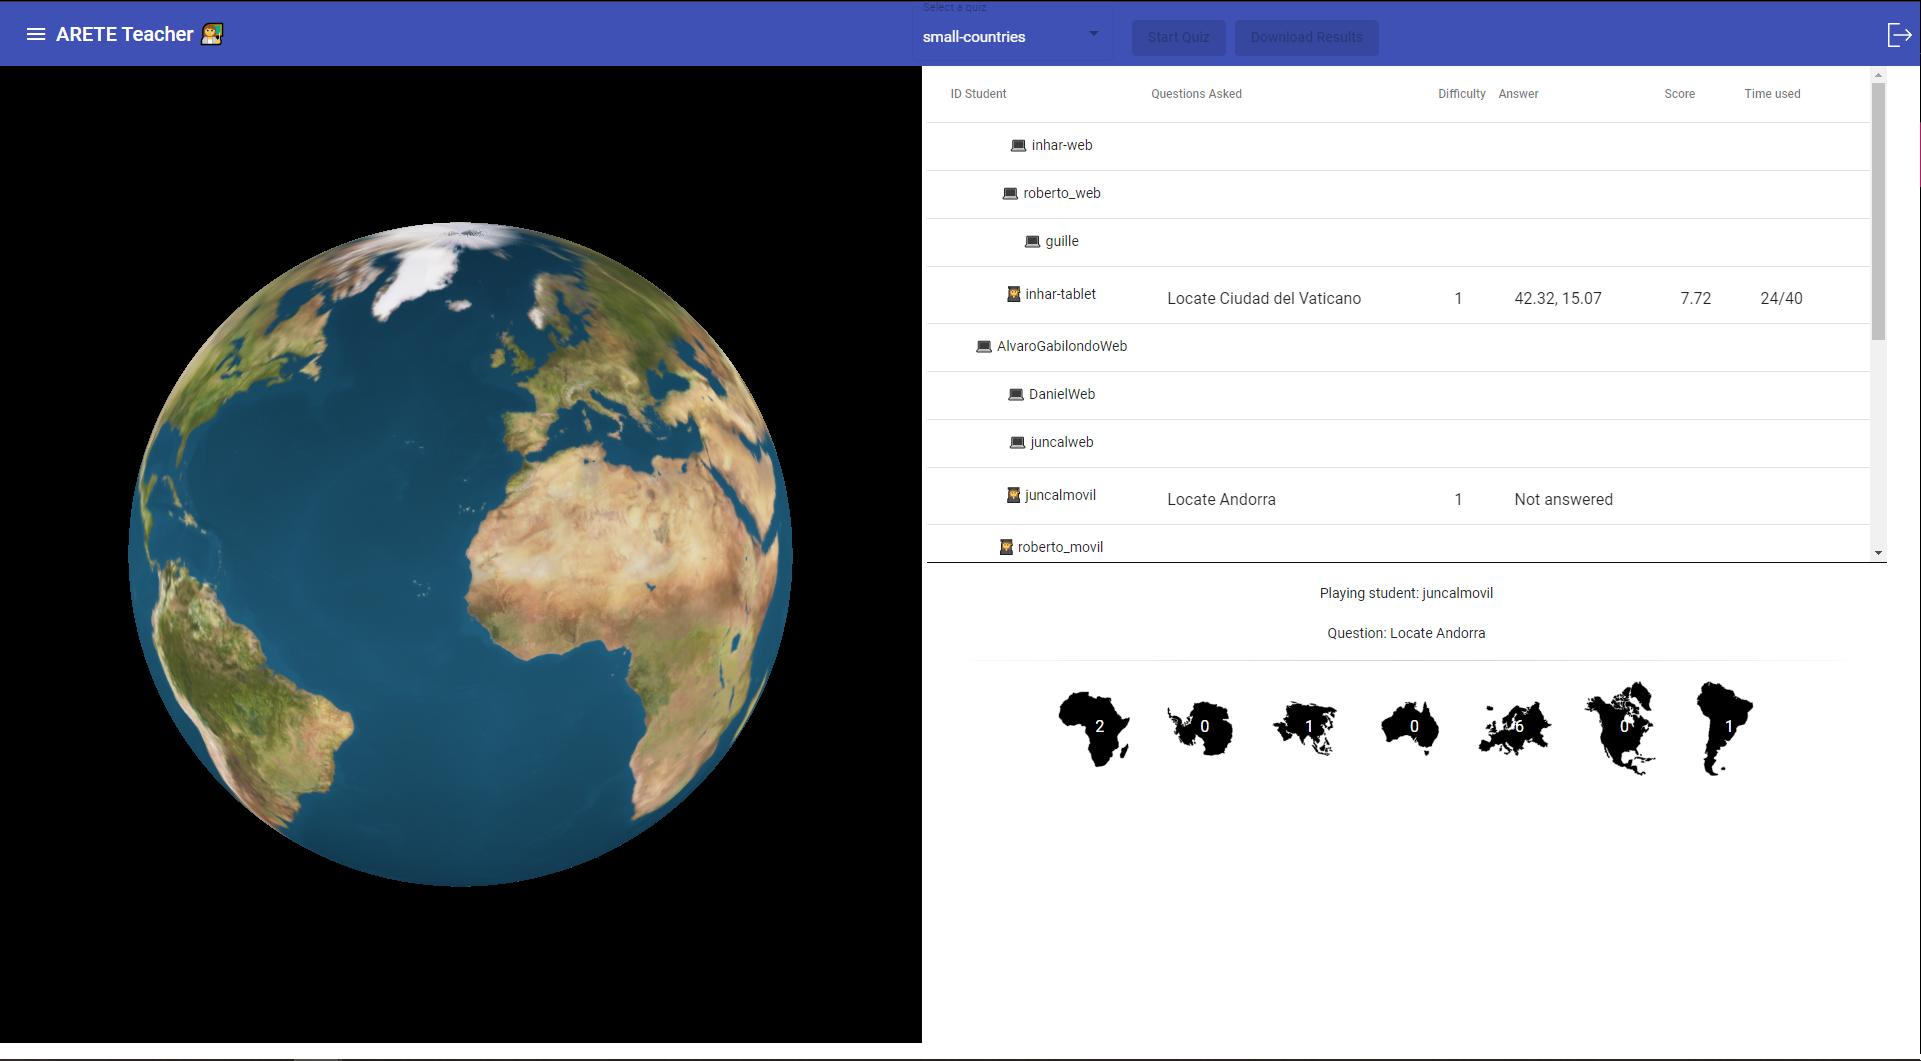
\includegraphics[width=0.95\textwidth]{Teacher_interface.png}
    \caption{\fontsize{10pt}{11pt}\selectfont{\itshape{The web-based teacher interface of the \appname{} application.}}}
    \label{fig:teacher_interface}
\end{figure*}

The application is designed to require minimal supervision from the teacher to let him or her interact as much as possible with the students.
As shown in Figure \ref{fig:teacher_interface}, the teacher interface consists of four parts:
\begin{itemize}
    \item A 3D representation of the augmented content as viewed by the active user (that is, the student who is answering the current question);
    \item The list of users connected to the app, together with the current score of the players and the last question they answered;
    \item The suggestions sent to the student currently answering the question;
    \item A dashboard (accessible in a separate tab) with charts of the scores achieved by each student across different sets of questions.
\end{itemize} 

The teachers who filled in the questionnaire described in Chapter \ref{chap:arch} mentioned that one of the factors limiting the usage of AR apps in schools is the lack of customisation capabilities.
In this respect, \appname{} provides an additional web interface from which the teacher can create new sets of questions.
To minimize the amount of work required by the teacher, the coordinates of each location are computed automatically using the Wikimedia API\footnote{\url{https://www.mediawiki.org/wiki/Wikimedia_REST_API}} and the questions are stored as JSON files, which are directly added to the application.
The interface of the \textit{watchers} is web-based, too, and has a look and feel similar to the teacher interface.

For the application to successfully achieve interoperability (\textbf{DO1}), several types of hardware as well as software libraries need to be supported.
In the aforementioned survey, the teachers reported a wide spectrum of devices available in their schools. Chromebooks and Android tablets were the most commonly used but other options included laptops, PCs, smartphones (both Android and iOS based) and iPads.
Furthermore, while none of the teachers reported using AR headsets such as HoloLens, it is believed that such devices provide the best AR learning experience for users. For this reason, the application supports Microsoft Mixed Reality Toolkit and is fully compatible with HoloLens devices.
The application for mobile and tablet devices has been developed using Unity 2020.3 and the AR functionalities are provided by the AR Foundation framework.
The web application has been built using Typescript and Three.js (to enable 3D content to be displayed in the browser). All the logging data and the statements collected during app usage are stored in a Mongo database in the Learning Locker instance deployed on AWS.
Porting to HoloLens and iOS devices is achieved through, respectively,  Unity integration with Microsoft MR Toolkit and by exporting the Unity project file to an XCode environment.

The application supports multi-user capabilities (\textbf{DO2}) by relying on the functionalities provided by the \arch{} architecture, which provides the \ork{} library for sharing 1-to-1 or broadcast message passing \citep{10.1007/978-3-030-93907-6_106} with minimal changes to the existing code base.
When a student is asked to answer a question, she becomes the active user. She shares the camera position (which determines her view of the 3D globe) as well as the position of the pin, once placed, with the other users.
The other students will then see, on their devices, the 3D globe in the same way the active user does.
For users on a mobile device this happens directly in the augmented space, while users using a PC will see the globe in a virtual 3D environment on a \texttt{\textless canvas\textgreater} element.
At the same time, suggestions from users are shared in a broadcast fashion, so that every student knows about the suggestions sent by others.
Finally, the teacher interface shares information about the current question, the score obtained by the active user after receiving her answer and the cumulative score of each user.
The information is shared 30 times per second and it allows a smooth \gls{ux} for every participant. The bandwidth usage is low since only basic data types such as strings and numbers are shared between users and the delay is below 15 milliseconds on both WiFi and mobile networks.
A previous approach tried to combine message passing and the transmission of the screen of the active user, using WebRTC, to the students using a PC to better simulate the AR experience \citep{UnityRenderStreaming}.
Unfortunately, such a solution has proven not to be scalable. Due to the poor support Unity has for WebRTC servers such as Janus, the application suffered delays which severely impacted the performance. With more than 5 users the UX was severely affected, and the app became unusable when more than 10 users were connected to the same session.

To comply with the data analytics design objectives (\textbf{DO3}, \textbf{DO4} and \textbf{DO5}) the application enables data collection through the storage of xAPI statements on a Learning Locker instance. 
Storing statements across each session enables the application to keep track of user activity and to store additional logging messages that simplify application debugging.
Learning Locker provides basic analytics and plotting capabilities through a web interface, as well as filtering and exporting the data in CSV format.
These functionalities have been extended through the development of a Python package\footnote{\url{https://stocastico.github.io/xapi_analysis/}} that includes methods to perform advanced data exploration and plotting, as well as running common machine learning models on xAPI statements data.
One of the aims of the package is to simplify data analysis as much as possible, enabling teachers without development skills to extract valuable information from the collected data.
For this reason, the package directly integrates GPT-4 \citep{openai2023gpt4, Osmulski_Ask_AI_-_2023}, so that users with a valid OpenAI Key can use natural language to debug or generate code when needed.
The package has been used to analyze the data collected during the evaluation of the app and the results will be presented in Section \ref{eval:results}.

Finally, to demonstrate how the aforementioned architecture enables developers to easily create multi-user applications (\textbf{DO6}), the developer of \appname{} was asked if and how the architecture helped him in the development process.
The developer mentioned that the architecture API enabled him to add multi-user functionalities in a transparent way. He neither had to deal with low-level networking issues nor implement platform specific methods.
While it was not possible to estimate the amount of lines of code or hours saved by using \arch{}, the developer said that he was satisfied with the capabilities of the architecture and would use it again for future projects.
Nevertheless, in order to enable teachers to create an ecosystem of collaborative AR applications for education, the developer mentioned that the availability of authoring tools to easily create applications on top of the \arch{} architectural design would be desirable.


%%%%%%%%%%%%%%%%%%%% EVALUATION %%%%%%%%%%%%%%%%%%%%%
\section{Evaluation}\label{eval:evaluation}

Our study aims to investigate how collaborative AR solutions may benefit the learning experience, and which are the usability issues of multi-user, multiplatform applications.
In the literature, unfortunately, there is no agreement on how to conduct evaluation of AR-based educational apps.
The survey from \cite{santos2013augmented} analyses 87 AR applications and the evaluation protocols included interviews, observing and coding overt behaviour and expert reviews.
Of those who used questionnaires, the majority crafted their own.
Among the works that used established questionnaires, some relied on the ISONORM Usability questionnaire \citep{prumper1999test}, Technology Acceptance Model \citep{davis1996critical}, Constructivist Multimedia Learning Environment Survey \citep{maor1999teacher}, Instructional Material Survey \citep{keller1987development}, Intrinsic Motivation Inventory \citep{ryan2000self}.
The number of participants in the evaluation of AR applications for education varies a lot depending on the study.
The systematic review of the literature published by \cite{masneri2020work}, of which Chapter \ref{chap:sota} represents an extension, shows that the number of participants varies between 2 and 290 participants. Another survey by \cite{santos2013augmented} analysed studies where the number of participants ranged from 4 to 419.

In this work, a questionnaire which adapts and extends the Positive System Usability Scale (P-SUS) \citep{brooke1996sus, sauro2011designing} was used. The questionnaire included a few additional questions to specifically evaluate the collaborative capabilities of the application.
The questions, presented in Appendix \ref{append:stuqu}, were grouped into 4 classes depending on what they were evaluating: the interest of the application as an educational tool, the usability of the app, its collaboration capabilities and its functionality.
Additionally, the participants could provide free-form feedback about the overall experience and whether they would recommend it to other students.
Finally, an interview with the teachers was conducted to collect their feedback about the learning experience, how collaboration may impact the involvement of the students, how  AR apps could be used to evaluate the students knowledge of a subject and how they would take advantage of the data collected through the application.

At the beginning of the evaluation, the participants were briefed about the experiment and its purpose and were asked to sign a consent form.
The questionnaires were anonymous but had an ID associated, so that during data analysis it was possible to associate the answers to the questionnaires with the data collected from each device through the xAPI statements.
The evaluation involved \numstudents/ students from \numschools/ educational institutions in San Sebastian (\textit{Colegio Salesianos Donostia}\footnote{\url{https://www.salesianosdonostia.com/es}}, \textit{IES Xabier Zubiri Manteo}\footnote{\url{https://zubirimanteo.hezkuntza.net/es/inicio}} and \textit{Universidad de Deusto}\footnote{\url{https://www.deusto.es/es/inicio}}) between March and May 2023.
Each experiment involved students of different ages (14, 17 and 19 years old) and their corresponding teachers.
None of the participants had previous experience with AR applications, but they were familiar with the hardware devices (smartphones, tablets and PCs) used during the evaluation.
In each school, the students were split into two groups: the first one represented the \textit{players}, tasked with answering the quiz questions using the application on mobile or tablet devices, while the second group represented the \textit{watchers}, who used a laptop or PC to see how the students answered the quiz and provided suggestions along the way.
Table \ref{tab:details_participants} shows the number of participants in each experiment, as well as details about the type of devices used when interacting with the application.

\begin{table*}[htbp]
\caption{\fontsize{10pt}{11pt}\selectfont{\itshape{Details of the demographics and number of devices used across each test.}}}
  \centering
  \begin{tabular}{l c c c c c c}
    \toprule
    \multirow{2}{*}{Participants} & \multicolumn{2}{c}{Gender} & \multicolumn{2}{c}{Players} & \multirow{2}{*}{Watchers} & \multirow{2}{*}{\textbf{Total}} \\
    \cmidrule(lr){2-3} \cmidrule(lr){4-5}
                            &  \multicolumn{1}{c}{Males} & \multicolumn{1}{c}{Females}  & \multicolumn{1}{c}{Tablets} & \multicolumn{1}{c}{Smartphones} & & \\
    \midrule
    14 year-old & 9 & 8 & 4 & 5 & 8 & \textbf{17} \\
    17 year-old & 16 & 1 & 3 & 6 & 8 & \textbf{17} \\
    19 year-old & 6 & 4 & 3 & 6 & 1 & \textbf{10} \\
    \midrule
    \textbf{Total} & \textbf{31} & \textbf{13} & \textbf{10} & \textbf{17} & \textbf{17} & \textbf{44}\\
    \bottomrule
  \end{tabular}
  \label{tab:details_participants}
\end{table*}

Once each participant had a device assigned, they were asked to connect to the application by selecting the session ID representing the experiment and the user ID. The latter would be used as the \textit{Actor} value for the xAPI statements generated while using the application.
After a short Q\&A session to clarify doubts about the app usage the teacher started the quiz and the students would then take turns to answer two sets of questions.
Once the quiz was over, the teacher stopped the data collection and was able to check the score of each student and to export the data.
After logging out of the session, the students filled in the questionnaires while the post-study interview with the teacher was conducted.


%%%%%%%%%%%%%%%%%%%% RESULTS %%%%%%%%%%%%%%%%%%%%%%%%
\section{Results and Discussion}\label{eval:results}

In this Section, the results of the survey as well as the data collected from the app are presented and discussed. An extended version which also includes a subgroup analysis of the data split for different age group, is available in the code and data repository\footnote{\url{https://github.com/Stocastico/Evaluation_paper}}. The quantitative results from the responses to the post-intervention survey (shown in Appendix \ref{append:stuqu}) are summarised in Figure \ref{fig:survey_all}. They are shown as stacked bar charts \citep{friedman1999rating}, where the chart on the left  refers to the answers to each question and the chart on the right to the groups of questions mentioned in Section \ref{eval:evaluation}.
From the figure it can be appreciated that the application was very well received by the students and that every question except the first one was answered positively (\textit{Agree} or \textit{Strongly agree}) more than 60\% of the time.
The average rating for each question ranges from $3.45$ to $4.43$, with limited variability across answers, with the standard deviation being below 1 for most of the questions.
The plot on the right in Figure \ref{fig:survey_all} shows similar results: the students assigned the highest score to questions related to Usability, especially question 2 (\textit{I found the application to be simple}) and 3 (\textit{I thought the application was easy to use}). The questions related to Functionality received a high score as well, while the ones relating to the Educational content of the app show the highest variability: those questions received the highest amount of negative answers while also receiving the highest score more than 40\% of the time. 

\begin{figure*}[htbp]
    \centering
    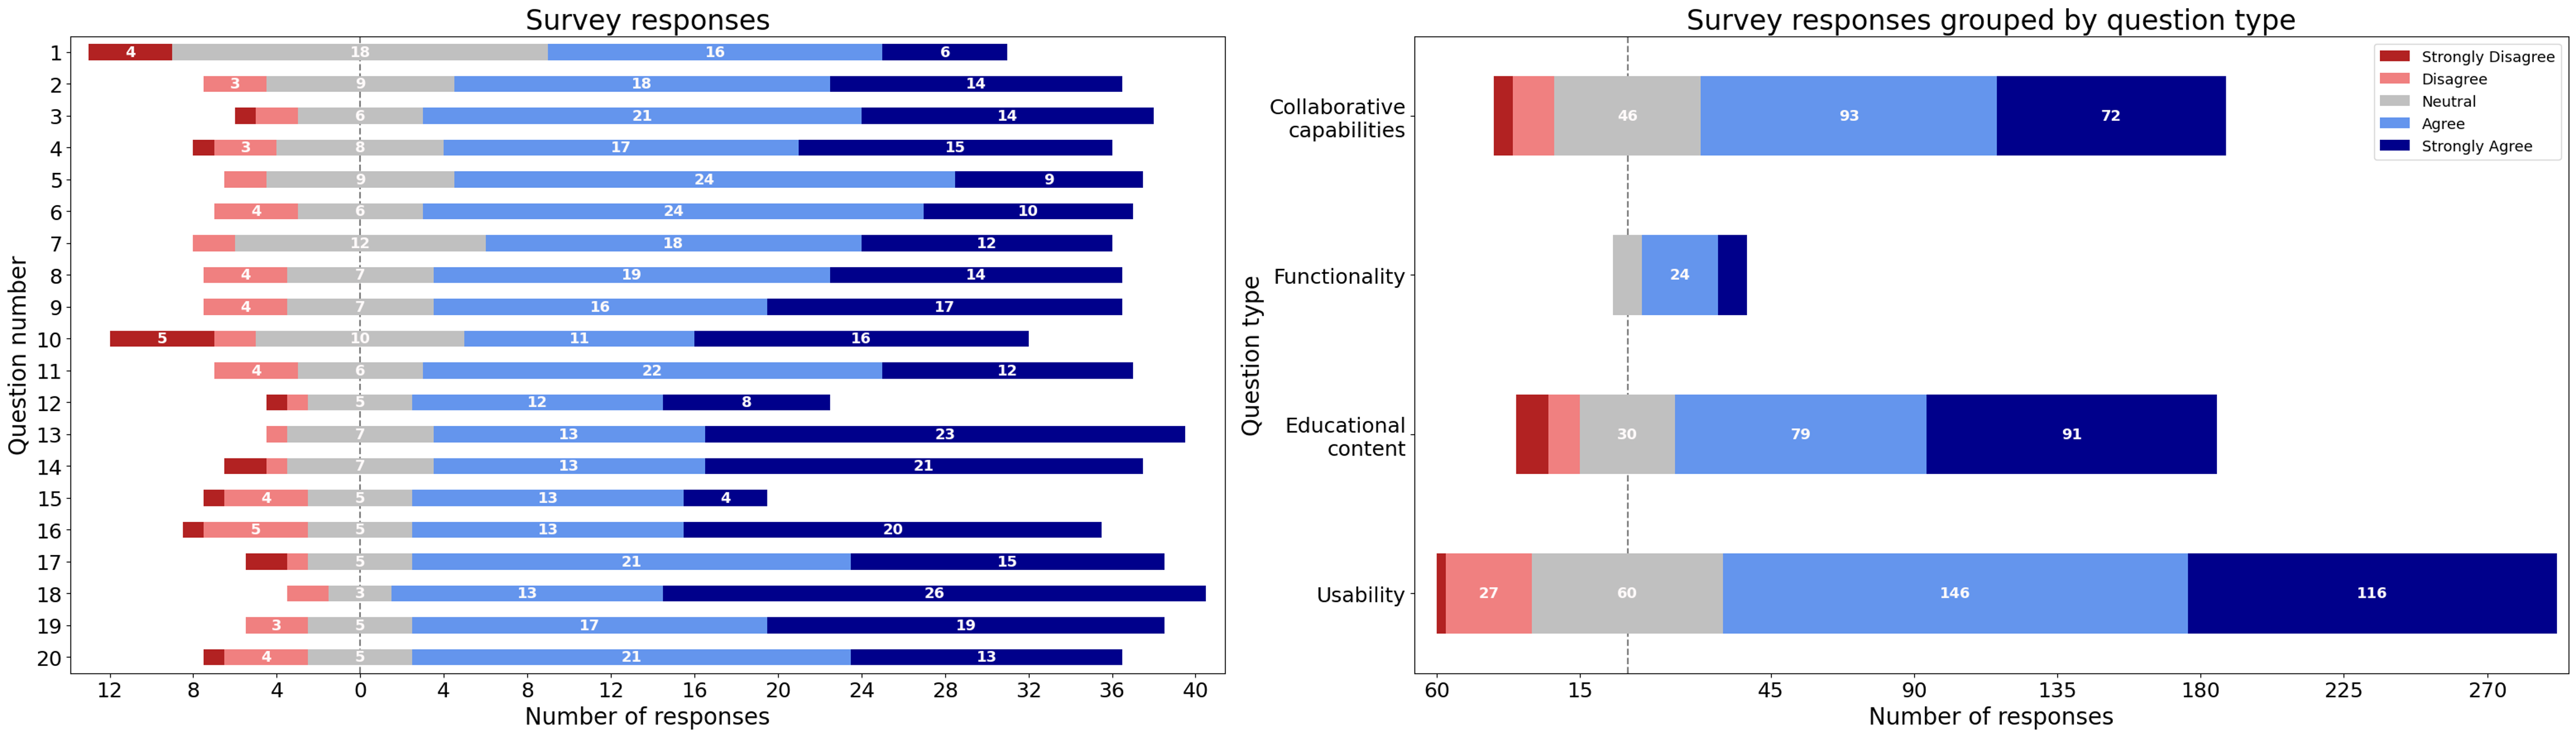
\includegraphics[width=0.95\textwidth]{survey_results_2.png}
    \caption{\fontsize{10pt}{11pt}\selectfont{\itshape{Left: survey results on each question. Right: survey results grouped by question type.}}}
    \label{fig:survey_all}
\end{figure*}

The bar plots of Figure \ref{fig:survey_split} are used to identify differences in the answers of the students, based on their role when using the app and the device they used.
Somewhat surprisingly the \textit{watchers} gave a slightly higher mean score, albeit with a much higher variability in the answer.
As for the device type, the users on an Apple device (iPhone or iPad) gave a higher score compared to students using an Android device or a PC, but the differences are not statistically relevant.

\begin{figure*}[htbp]
    \centering
    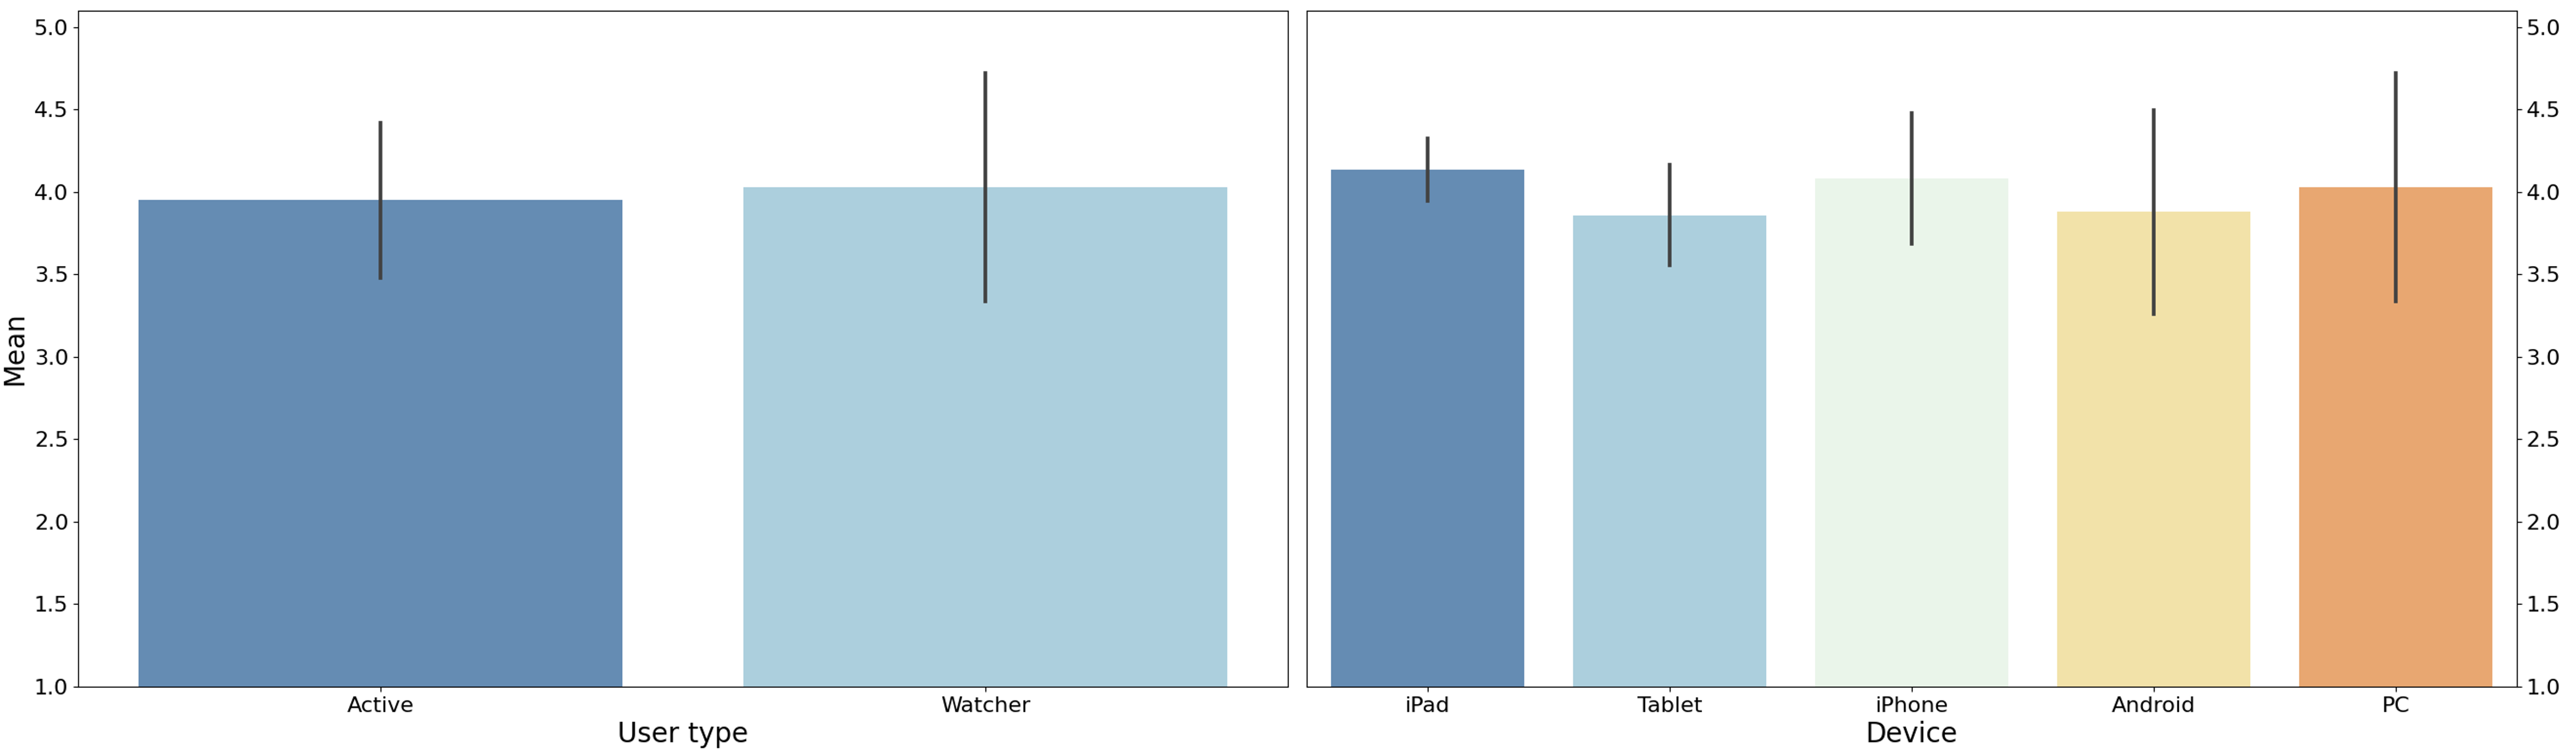
\includegraphics[width=0.95\textwidth]{survey_results_type_2.png}
    \caption{\fontsize{10pt}{11pt}\selectfont{\itshape{Mean score of the questionnaire answers. The vertical bars represent the standard deviation.}}}
    \label{fig:survey_split}
\end{figure*}

Figure \ref{fig:survey_split_grouped} shows the mean score and the standard deviation for the questionnaire answers grouped by user.
It shows the split of the students by age, their role when using the app and the device they used.
From this visualization an outlier can be easily identified, represented by the only student in the 19 year-old group who used a PC and was the only non-active user in that session.
The reason for the lower score, as identified by the comments provided by the student in the questionnaire, was that the experience for him did not feel particularly immersive nor collaborative, as his role was fairly different from that of his classmates. 

\begin{figure*}[htbp]
    \centering
    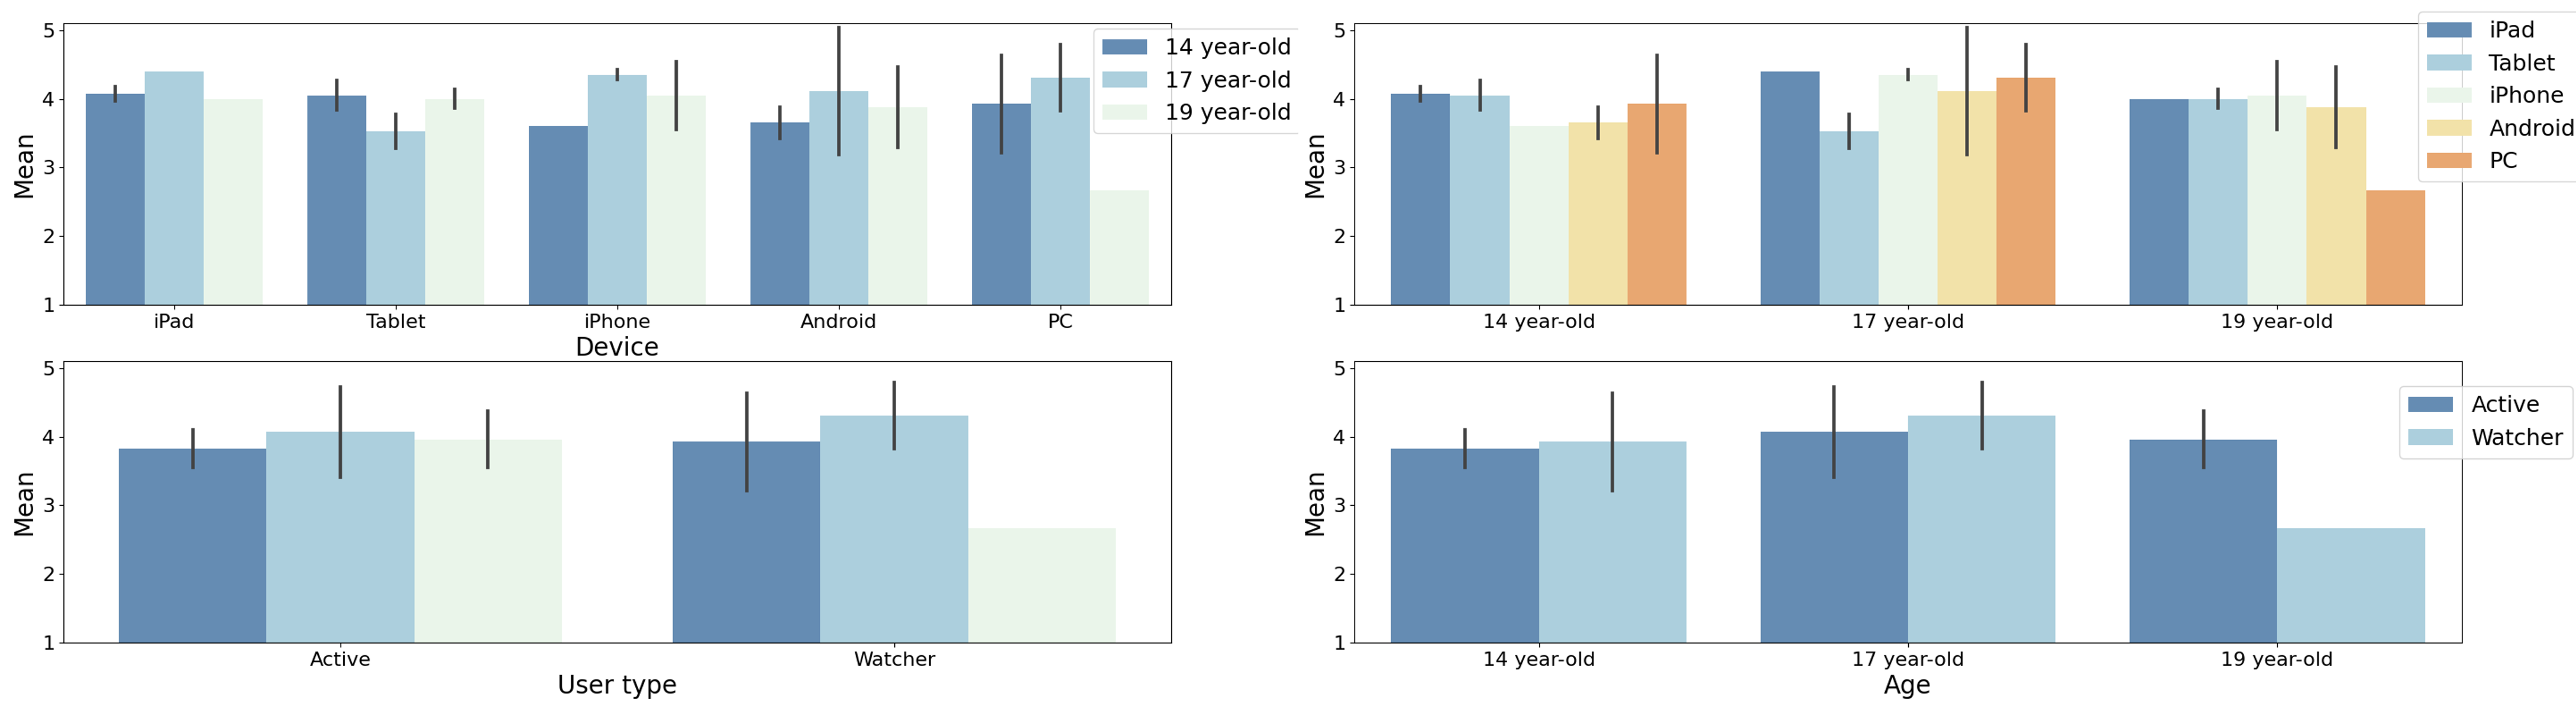
\includegraphics[width=0.95\textwidth]{survey_results_grouped_2.png}
    \caption{\fontsize{10pt}{11pt}\selectfont{\itshape{Survey results split by user type. Left: Average question score by device used and student role. Right: Average question score by students age.}}}
    \label{fig:survey_split_grouped}
\end{figure*}

Since \appname{} collected data in the form of xAPI statements, an analysis of the data received was conducted. This showed that there is a correlation between the score in the questionnaire and the number of statements collected by the application for each user.
The actions registered by the app include both interactions between students, such as the suggestions sent, and the interactions of a user with the app.
As shown in Figure \ref{fig:num_interactions}, there is a high variability in how much the students interacted. It is clear, though, that the \textit{players} (the students using a mobile device and interacting with the augmented content) were much more involved in using \appname{}. This is probably because their role was much more interactive and immersive.

\begin{figure}[htbp]
    \centering
    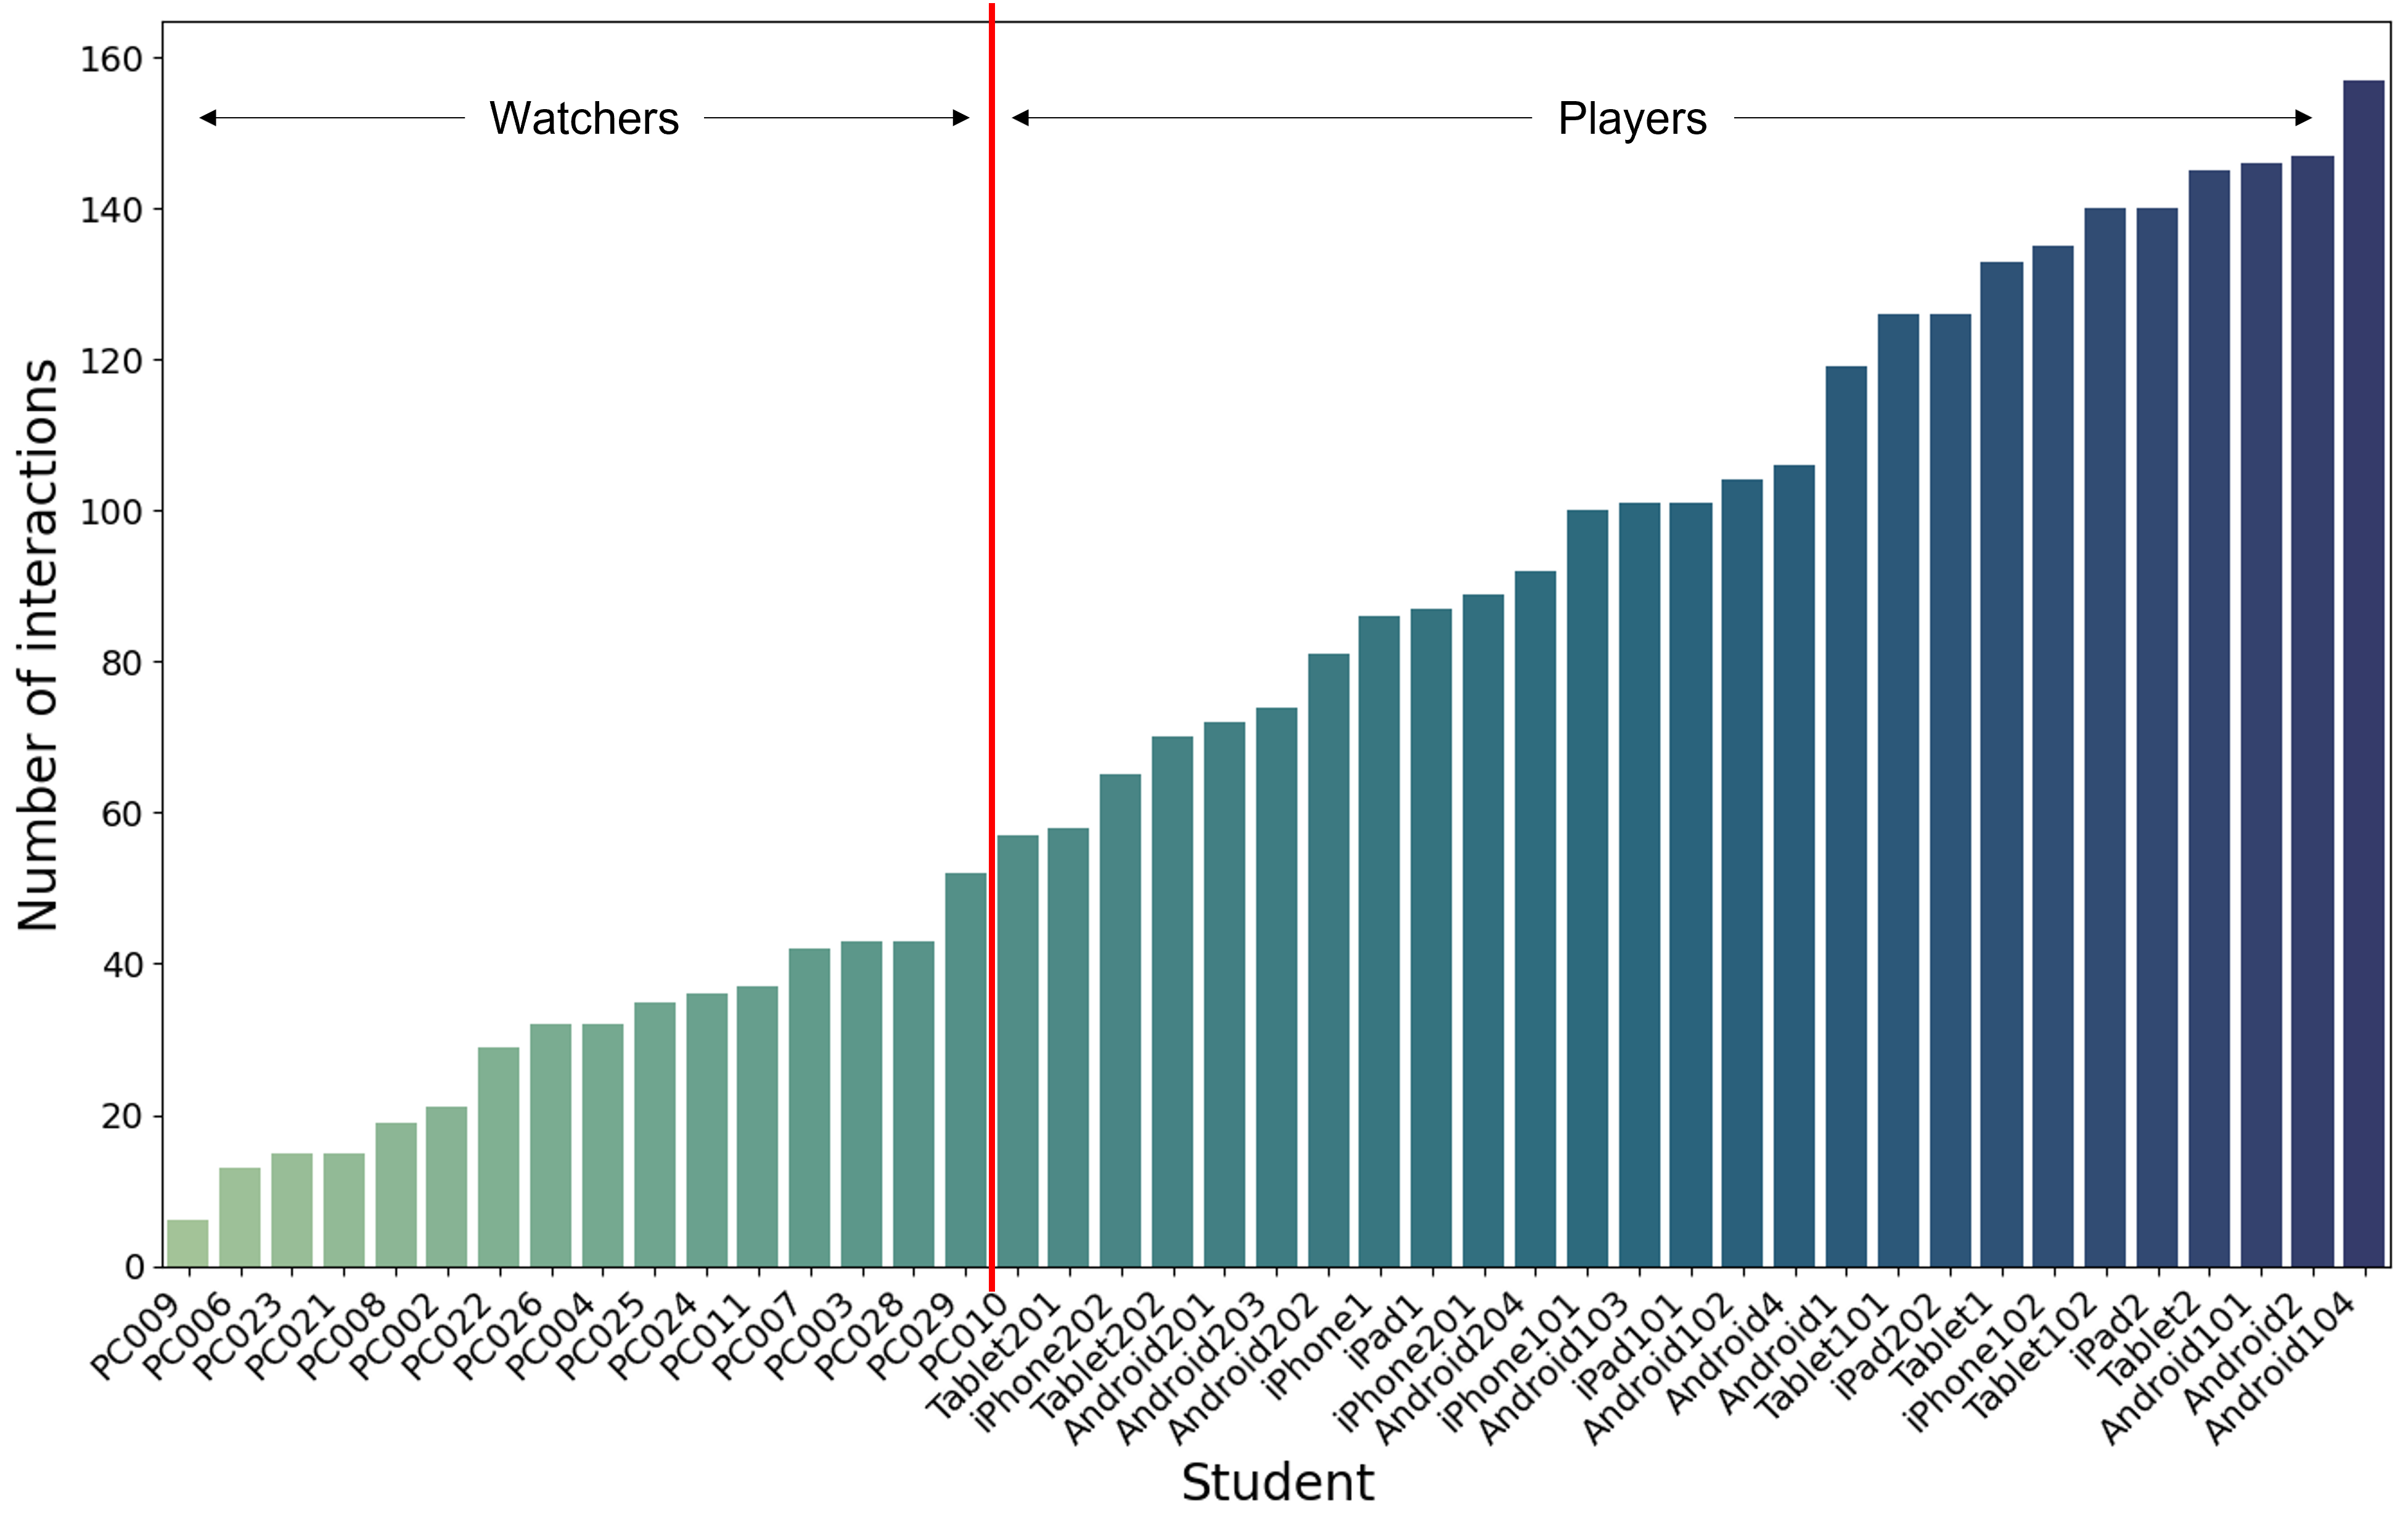
\includegraphics[width=0.95\textwidth]{num_interactions_2.png}
    \caption{\fontsize{10pt}{11pt}\selectfont{\itshape{Interactions with the application for each student (identified by the device used).}}}
    \label{fig:num_interactions}
\end{figure}

An interesting aspect to analyse is whether there is any correlation between the number of interactions of each student and the answers they have given to the survey questions.
Two statistical approaches were followed.
First,  a correlation analysis was performed to check whether there was a relation between the number of interactions and the average scores given to the questions by the students, by calculating the Pearson correlation coefficient.
The second approach is that of hypothesis testing. This checks whether the answers given by students with a high number of interactions are significantly different from the answers given by students who had a low number of interactions.
A two-sample T-test assuming equal variances has been used for testing \citep{welch1947generalization}.
In both cases, a significance level of $p < 0.05$ was established.
Since the interactions between the \textit{watchers} (students on a PC) and \textit{players} (students on a mobile device) are significantly different, it was also performed an analysis for these specific subsets of the data as well.

Unfortunately, the analysis performed is not conclusive.
None of the tests returned a p-value below the significance level, and the correlations identified (most notably between the interactions of students on a PC and their answers to the survey) are not statistically significant.

A similar analysis was conducted to inspect whether there were correlations between the score obtained in the quiz and the answers in the survey. In this case as well, no statistically significant correlation was found.
This was  expected since the app was designed to ask questions of varying difficulties, but the difficulty level of the questions received by a student did not change during the test.
As expected, students who received easier questions achieved a higher score and there is indeed a significant correlation between these two variables.

Another interesting correlation to analyse was the one between the mean score obtained in the survey and the number of suggestions sent by the user.
The statements about suggestions are an interesting variable because for each question, every user (besides the \textit{active player}, the one answering the current question) was able to send two suggestions.
For this reason, many such statements were collected during the trial.
To encourage students to provide suggestions, the application assigned points for each correct suggestion.
In this case the analysis showed a significant positive correlation ($r = .37$, $p = .044$), meaning that the most engaged students were the ones that gave a higher score in the survey.

Finally, a clustering analysis of the data was performed, to check if it is possible to identify distinct groups of users.
In this case, the focus was only on the students who used a mobile device, since they provided a greater number of features to work with.
The average time left per question, the number of suggestion accepted, the total number of interactions and the mean value of the answers in the survey were the four variables considered.
A dimensionality reduction using PCA \citep{jolliffe2002principal}, shown on the left in Figure \ref{fig:clustering}, revealed that the first two principal components explained more than 70\% of the variance in the data.
Additionally, a biplot analysis indicated that the most relevant variable for the first principal component was the number of user interactions, while for the second one it was the results of the survey.

As the number of data points is small, a hierarchical clustering algorithm \citep{hiera} was used.
A Silhouette score \citep{ROUSSEEUW198753} computed for cuts between 2 and 6 suggested that the optimal number of clusters in this case was either 2 or 4.
The clustering results (shown in Figure \ref{fig:clustering}, right) identified one big group of students characterized by having a particularly high number of interactions and another one having a higher score in the survey answer.
The other two clusters were harder to characterise.
In one case it was not possible to clearly identify a common feature in the data, while in the other the cluster only contained two members, and the intra-cluster variable suggests that those data points are probably outliers.

After running the trials in the educational institutions, a post-intervention interview with the teachers was conducted.
The 3 teachers seemed very intrigued by the possibility of easily being able to use AR in school without having to resort to any specific hardware. They especially valued the fact that the collaborative features of \appname{} encouraged the students to work together to provide the answer, either through the features of the application or simply by talking to each other.
Another relevant point for the teachers was the possibility of adding new content on their own, as well as the fact that they could export the results to the school \gls{lms}.
The teachers were more sceptical about the AI features provided by the backend. They mentioned that the vast majority of their colleagues do not have sufficient knowledge to perform the analysis on their own. They would rather prefer using a PowerBI or Tableau interface to visualise data and extract basic reports.
The teachers also mentioned that the role of the \textit{watchers} was too passive and that in longer experiments these students might lose interest. They suggested enabling the role of active user when using a PC, even if that means not using AR components but a browser-based 3D graphics library.

\begin{figure*}[htbp]
    \centering
    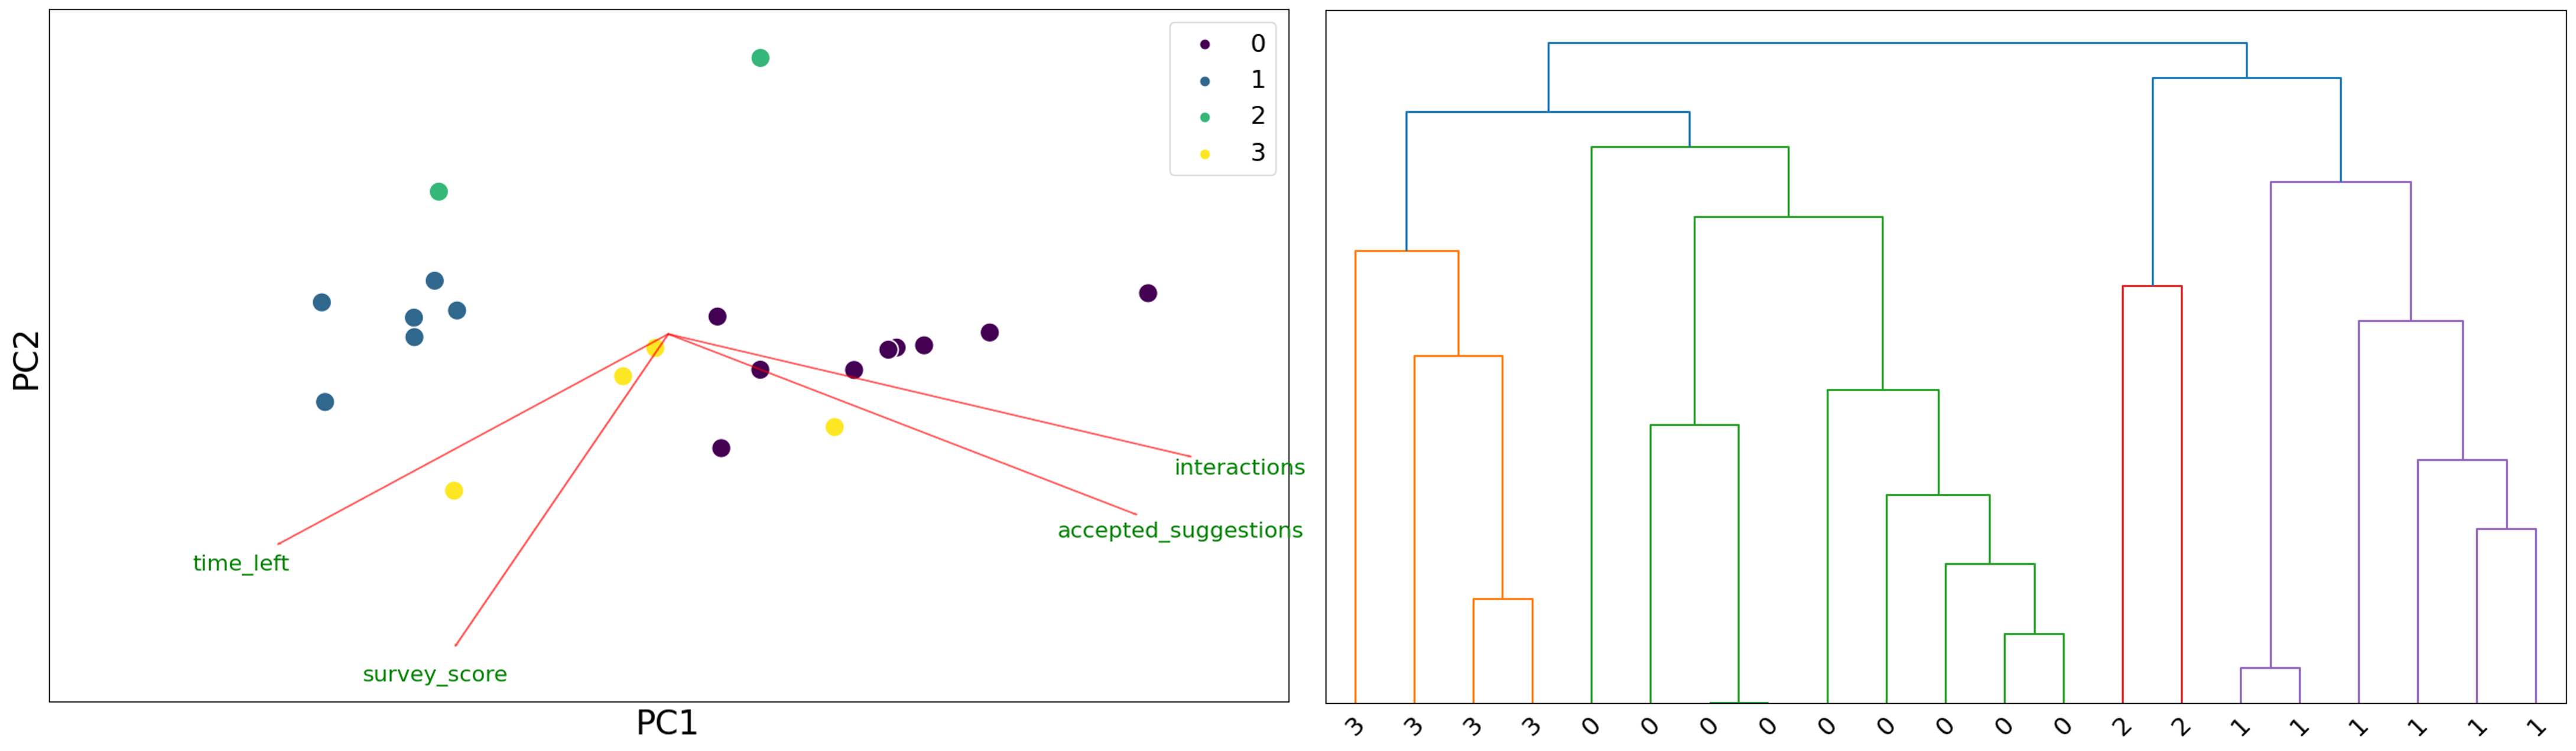
\includegraphics[width=0.95\textwidth]{unsup_3.png}
    \caption{\fontsize{10pt}{11pt}\selectfont{\itshape{Left: Clustering of the active users data on the PCA space. Right: the dendrogram representing the hierarchical clustering.}}}
    \label{fig:clustering}
\end{figure*}

%%%%%%%%%%%%%%%%%%%% CONCLUSIONS %%%%%%%%%%%%%%%%%%%%
\section{Final remarks}\label{eval:conclusion}

In this Chapter, \appname{} was presented, a multiplatform AR application which implements collaborative capabilities and gamification concepts. The application is based on a Geography quiz and it fulfils the design objectives identified in Chapter \ref{chap:arch}.
The evaluation, conducted with 44 students and 3 teachers, and the analysis of the xAPI statements showed that students evaluated very positively the application.
Additionally, it was measured a small but statistically significant correlation between the ratings in the questionnaire and the engagement of the students. Furthermore, post-study interviews with the teachers identified the collaborative capabilities and the possibility of personalising the app content as being key factors for a sustained usage of AR apps.
In fact, one of the teachers suggested the possibility of adding more collaborative features, such as a chat system or speech-based interactions to make the application more immersive and more appealing when used in a distributed setting.




